\documentclass[12pt, a4paper]{article}
\usepackage[a4paper,top=1.5cm, bottom=1.5cm, left=2cm, right=2cm]{geometry}
\usepackage{graphicx} % Required for inserting images
%%% Работа с русским языком
\usepackage{cmap}					% поиск в PDF
\usepackage{mathtext} 				% русские буквы в фомулах
\usepackage[T2A]{fontenc}			% кодировка
\usepackage[utf8]{inputenc}			% кодировка исходного текста
\usepackage[english,russian]{babel}	% локализация и переносы
\usepackage{float}
\usepackage{subcaption}
\usepackage{wrapfig}
\usepackage{tabularx}
\usepackage{multirow}

\usepackage[unicode, colorlinks=true, urlcolor=blue]{hyperref}
\usepackage[rgb]{xcolor}
\hypersetup{
colorlinks=true,urlcolor=blue
}
%%% Дополнительная работа с математикой
\usepackage{amsmath,amsfonts,amssymb,amsthm,mathtools} % AMS
\usepackage{icomma} % "Умная" запятая: $0,2$ --- число, $0, 2$ --- перечисление
%% Номера формул
\mathtoolsset{showonlyrefs=true} % Показывать номера только у тех формул, на которые есть \eqref{} в тексте.
%% Шрифты
\usepackage{euscript}	 % Шрифт Евклид
\usepackage{mathrsfs} % Красивый матшрифт
%% Свои команды
\DeclareMathOperator{\sgn}{\mathop{sgn}}
%% Перенос знаков в формулах (по Львовскому)
\newcommand*{\hm}[1]{#1\nobreak\discretionary{}
{\hbox{$\mathsurround=0pt #1$}}{}}


\usepackage{indentfirst}
\usepackage{amsmath,amssymb}
\usepackage[italicdiff]{physics}
\graphicspath{{images/}}
\DeclareGraphicsExtensions{.pdf,.png,.jpg}
\usepackage{enumitem}
\usepackage{caption}
\usepackage{array}
\usepackage{ragged2e}







\begin{document}



\include{titlepage}
\begin{titlepage}
\thispagestyle{empty}

\begin{center}
\small
Министерство науки и высшего образования Российской Федерации\\[2mm]
\textbf{ФЕДЕРАЛЬНОЕ ГОСУДАРСТВЕННОЕ АВТОНОМНОЕ
ОБРАЗОВАТЕЛЬНОЕ УЧРЕЖДЕНИЕ ВЫСШЕГО ОБРАЗОВАНИЯ}\\[1mm]
«МОСКОВСКИЙ ФИЗИКО-ТЕХНИЧЕСКИЙ ИНСТИТУТ\\
(НАЦИОНАЛЬНЫЙ ИССЛЕДОВАТЕЛЬСКИЙ УНИВЕРСИТЕТ)»\\
(МФТИ, Физтех)
\end{center}

\vspace{18mm}

\begin{center}
\large \textbf{КАФЕДРА ЭЛЕКТРОНИКИ}\\[10mm]
\Large \textbf{ОТЧЁТ}\\[2mm]
\large \textbf{ПО ЛАБОРАТОРНОЙ РАБОТЕ}\\[14mm]
\Large \textbf{РАСТРОВЫЙ ЭЛЕКТРОННЫЙ МИКРОСКОП}
\end{center}

\vfill

% Блоки с подписями слева, линии и пояснения справа
\noindent
\begin{tabular}{@{}p{0.44\linewidth}p{0.52\linewidth}@{}}
\textit{Работу выполнили:} & Акимов Михаил,

Новиков Василий,

Рагозина Елизавета,

Струков Олег,

Топольский Михаил,

Группа Б04-404 \\[8mm]

\textit{Работу принял, оценка:} & \\[3mm]
 \\
\end{tabular}


\vspace{12mm}

\begin{center}
\small Долгопрудный, \the\year{}~г.
\end{center}

\end{titlepage}










\newpage

\section*{Теоретическая часть}

\subsection*{Принцип действия растрового электронного микроскопа}

Растровый электронный микроскоп (РЭМ) представляет собой прибор, позволяющий исследовать поверхность образцов с высоким разрешением за счёт сканирования тонким сфокусированным пучком электронов. Принцип действия РЭМ основан на регистрации вторичных электронов, возникающих при взаимодействии первичного электронного зонда с поверхностью образца.

Основное преимущество РЭМ перед оптическими микроскопами заключается в значительно большем разрешении, достигающем 1~нм и менее. Это обусловлено малой длиной волны де~Бройля для электронов с энергиями в диапазоне 1--30~кэВ.

\subsection*{Вторичная электронная эмиссия}

При бомбардировке поверхности образца первичными электронами происходит испускание вторичных электронов --- явление, называемое вторичной электронной эмиссией (ВЭЭ). Энергетический спектр вторичных электронов можно разделить на три характерные области:

\begin{itemize}
    \item \textbf{Область~I} --- истинно вторичные электроны с энергиями $0 < E < 50$~эВ. Эти электроны возникают в результате ионизации атомов вещества первичным пучком. Отношение числа истинно вторичных электронов к числу первичных электронов называют коэффициентом истинно вторичной эмиссии $\delta$.    
    \item \textbf{Область~II} --- неупругоотражённые первичные электроны с энергиями $50$~эВ $< E < E_0$, где $E_0$ --- энергия первичных электронов.   
    \item \textbf{Область~III} --- упругоотражённые первичные электроны с энергиями, близкими к $E_0$. Коэффициент упругого отражения $R$ обычно не превышает 10\% при $E_0 > 50$~эВ.
\end{itemize}

\begin{figure}[h]
    \centering
    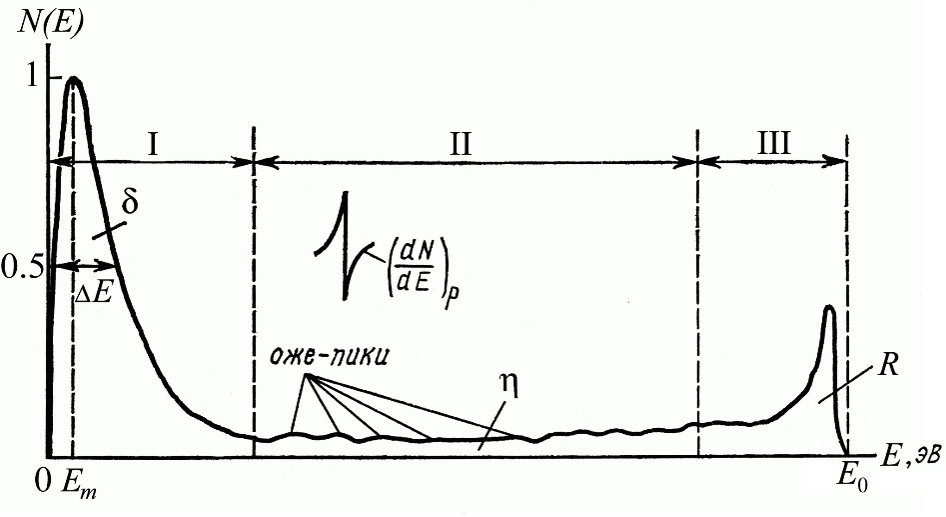
\includegraphics[width=0.6\textwidth]{1.png}
    \caption{Энергетический спектр вторичных электронов}
    \label{fig:spectrum}
\end{figure}

% Коэффициент вторичной эмиссии $\delta$ зависит от: энергии первичных электронов $E_0$; атомного номера материала образца $Z$; угла падения первичного пучка; состояния поверхности образца.


\subsection*{Генерация рентгеновского излучения и оже-эффект}

При бомбардировке вещества первичными электронами возникает характеристическое рентгеновское излучение. Электрон с энергией в несколько кэВ выбивает электрон с внутренней $K$- или $L$-оболочки, образуя вакансию, которая заполняется электроном с вышележащего уровня с испусканием рентгеновского кванта. Энергия этого излучения подчиняется закону Мозли:
\begin{equation}
    \sqrt{\nu} = K(Z - \sigma),
\end{equation}
где $Z$ --- атомный номер элемента, а $K$ и $\sigma$ --- константы. Эффективность возбуждения рентгеновского излучения электронным ударом составляет лишь $\sim 0,001$. Низкая эффективность обусловлена преимущественным взаимодействием зонда с внешними электронами атома, наличием тормозного фона, а также конкуренцией с безызлучательным переходом --- оже-эффектом.

\begin{figure}[h]
    \centering
    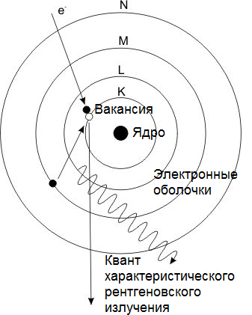
\includegraphics[width=0.3\textwidth]{2.png}
    \caption{Схема образования характеристического рентгеновского излучения и оже-электрона}
    \label{fig:xray}
\end{figure}

Альтернативным путём релаксации возбуждённого атома является образование \textbf{оже-электронов}. При переходе электрона на нижний уровень освободившаяся энергия передаётся не в виде фотона, а третьему электрону из той же или вышележащей оболочки. Если эта энергия превышает работу выхода, электрон покидает вещество. Энергия оже-электронов также строго зависит от атомного номера элемента, что позволяет использовать их для элементного анализа. Однако из-за крайне малой глубины выхода (единицы нанометров) оже-спектроскопия чувствительна лишь к самым поверхностным слоям образца.


\subsection*{Устройство электронной пушки}

Источником электронов в РЭМ служит электронная пушка. В приборе JOEL JSM-7001F используется вольфрамовый термополевой катод. Электронная пушка состоит из трёх электродов:
\begin{enumerate}
    \item \textbf{Катод} --- вольфрамовая нить, нагреваемая до температуры $T \approx 2800$~К для термоэмиссионных катодов или $T \approx 1800$~К для термополевых.
    
    \item \textbf{Цилиндр Венельта} --- управляющий электрод, на который подаётся отрицательное напряжение смещения относительно катода. Цилиндр Венельта регулирует ток эмиссии и фокусирует электроны.
    
    \item \textbf{Анод} --- заземлённая пластина с отверстием диаметром около 2~мм, расположенная на расстоянии $\approx 10$~мм от цилиндра Венельта. На участке между цилиндром Венельта и анодом происходит ускорение электронов до энергий 1--30~кэВ.
\end{enumerate}

\begin{figure}[h]
    \centering
    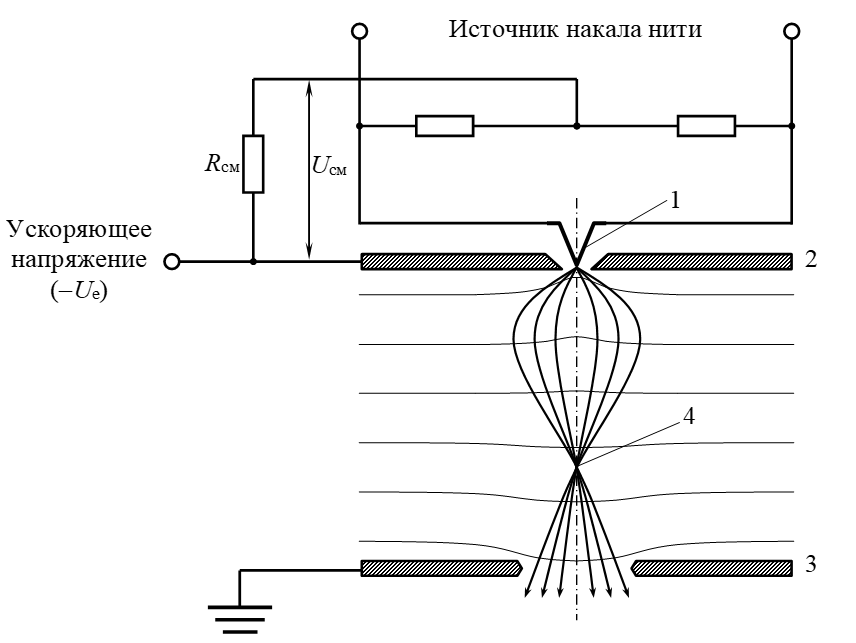
\includegraphics[width=0.5\textwidth]{3.png}
    \caption{Схема трёхэлектродной электронной пушки: 1 --- катод, 2 --- венельт, 3 --- анод, 4 --- кроссовер}
    \label{fig:gun}
\end{figure}

В пространстве между цилиндром Венельта и анодом пучок сужается, образуя \textbf{кроссовер} --- минимальное сечение пучка. Диаметр кроссовера определяется тепловым разбросом скоростей электронов и зависит от: температуры катода $T_k$; ускоряющего напряжения $V_a$; фокусного расстояния пушки.


% Радиус кроссовера можно оценить по формуле:
% \begin{equation}
%     r_c \approx r_k \sqrt{\frac{kT_k}{eV_a}},
% \end{equation}
% где $r_k$ --- радиус излучающей поверхности катода.

\subsection*{Электронная оптика}

После выхода из электронной пушки электроны попадают в систему электромагнитных линз, формирующих узкий зонд на поверхности образца. Магнитная линза представляет собой соленоид с острыми кольцевыми наконечниками полюсов, создающий сильное неоднородное магнитное поле.

% Механизм фокусировки в магнитной линзе:
% \begin{itemize}
%     \item горизонтальная компонента магнитного поля сообщает электрону азимутальную скорость;
%     \item вертикальная компонента поля создаёт радиальную силу Лоренца, направленную к оси;
%     \item в результате электроны отклоняются к оптической оси, аналогично преломлению света в оптической линзе.
% \end{itemize}

\begin{figure}[h]
    \centering
    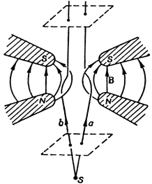
\includegraphics[width=0.2\textwidth]{4.png}
    \caption{Движение электронов в магнитной линзе}
    \label{fig:lens}
\end{figure}

% Электронно-оптическая система РЭМ JOEL JSM-7001F содержит:
% \begin{itemize}
%     \item \textbf{две конденсорные линзы} --- для фокусировки пучка и регулировки тока зонда;
%     \item \textbf{сменную диафрагму} --- для ограничения апертуры пучка;
%     \item \textbf{сканирующие катушки} --- для отклонения пучка при сканировании;
%     \item \textbf{объективную линзу} --- для окончательной фокусировки зонда на образце.
% \end{itemize}

% Объективную линзу располагают как можно ближе к образцу для достижения максимальной фокусировки. Однако это ограничивает возможности размещения детектирующей аппаратуры.

\subsection*{Формирование изображения}

Изображение в РЭМ формируется растровым способом: электронный зонд последовательно сканирует поверхность образца точка за точкой. Отклонение пучка осуществляется с помощью электромагнитных катушек, создающих поперечное магнитное поле.

На отклоняющие катушки подаётся пилообразное напряжение развёртки, аналогично телевизионной системе. Сигнал с детектора вторичных электронов модулирует яркость соответствующей точки на экране монитора.

\begin{figure}[h]
    \centering
    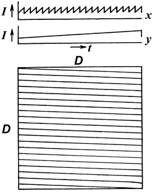
\includegraphics[width=0.2\textwidth]{5.png}
    \caption{Схема формирования растра при сканировании}
    \label{fig:scanning}
\end{figure}

Качество изображения характеризуется отношением сигнал/шум:
\begin{equation}
    \frac{S}{N} = \frac{n}{\sqrt{n}} = \sqrt{n},
\end{equation}
где $n = \delta n_p$ --- число вторичных электронов, регистрируемых с одной точки, $\delta$ --- коэффициент вторичной эмиссии, $n_p$ --- число первичных электронов.

Число первичных электронов определяется:
\begin{equation}
    n_p = \frac{j \cdot t \cdot \pi d^2}{4e},
\end{equation}
где $j$ --- плотность тока зонда, $d$ --- диаметр зонда, $t$ --- время накопления сигнала в точке, $e$ --- заряд электрона.

Для улучшения отношения сигнал/шум при малых токах зонда увеличивают время сканирования, однако это приводит к удлинению времени получения изображения.

% \subsection*{Разрешающая способность РЭМ}

% Пространственное разрешение РЭМ определяется несколькими факторами:
% \begin{enumerate}
%     \item \textbf{Диаметр электронного зонда} --- зависит от яркости источника, аберраций линз и дифракции.
    
%     \item \textbf{Область взаимодействия} --- электроны рассеиваются внутри образца, и пучок «расплывается». Характерный размер области генерации вторичных электронов составляет 0,5--5~мкм в зависимости от энергии электронов и материала образца.
    
%     \item \textbf{Ускоряющее напряжение} --- при увеличении энергии электронов диаметр зонда уменьшается, но пучок глубже проникает в образец и сильнее расширяется за счёт рассеяния.
% \end{enumerate}

% \begin{figure}[h]
%     \centering
%     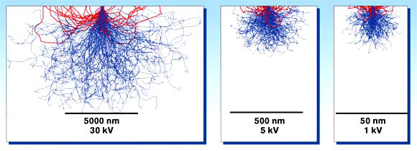
\includegraphics[width=0.7\textwidth]{6.png}
%     \caption{Зависимость области взаимодействия от ускоряющего напряжения}
%     \label{fig:resolution}
% \end{figure}

% На практике находят компромисс между этими факторами. Типичные значения ускоряющего напряжения составляют 5--20~кэВ, при этом разрешение достигает 1--10~нм для современных приборов.

% \subsection*{Детектирование рентгеновского излучения}

% Для элементного микроанализа в РЭМ используют два типа детекторов рентгеновского излучения:

% \textbf{Волновой (дифракционный) детектор} основан на законе Брегга–Вульфа:
% \begin{equation}
%     n\lambda = 2d\sin\theta,
% \end{equation}
% где $d$ --- межплоскостное расстояние кристалла-анализатора, $\theta$ --- угол падения, $n$ --- порядок интерференции.

% Кристалл-анализатор и детектор располагаются на круге Роуланда. Спектральное разрешение волнового детектора составляет 10--15~эВ, однако быстродействие невелико из-за необходимости механического перемещения кристалла.

% \textbf{Энергодисперсионный детектор} (Si(Li) или HpGe) преобразует энергию каждого фотона в пропорциональный электрический сигнал. Детектор охлаждается жидким азотом до 77~К для снижения шумов. Спектральное разрешение составляет $\approx 120$~эВ, но быстродействие на порядки выше, чем у волнового детектора.

% \begin{figure}[h]
%     \centering
%     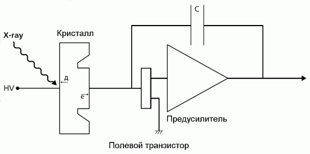
\includegraphics[width=0.65\textwidth]{7.png}
%     \caption{Схема энергодисперсионного детектора}
%     \label{fig:eds}
% \end{figure}

% \subsection*{Количественный микроанализ}

% Для определения концентрации элементов в образце сравнивают интенсивность характеристического излучения $I$ с интенсивностью $I_0$ эталонного образца:
% \begin{equation}
%     \frac{C}{C_0} = \frac{I}{I_0},
% \end{equation}
% где $C$ и $C_0$ --- концентрации элемента в образце и эталоне соответственно.

% Однако эта простая формула не учитывает эффекты:
% \begin{itemize}
%     \item \textbf{атомного номера ($Z$)} --- различие в тормозной способности и обратном рассеянии;
%     \item \textbf{поглощения ($A$)} --- поглощение рентгеновского излучения в образце;
%     \item \textbf{флуоресценции ($F$)} --- возбуждение излучения одного элемента характеристическим излучением другого.
% \end{itemize}

% Поэтому применяют \textbf{ZAF-коррекцию}, вводя эмпирические поправочные коэффициенты. Предел обнаружения примесей при количественном микроанализе составляет $\approx 0{,}001$\%.

% \subsection*{Виды катодов и их характеристики}

% По типу эмиссии катоды РЭМ делятся на:
% \begin{enumerate}
%     \item \textbf{Термоэмиссионные} (W, LaB$_6$) --- температура накала $T \approx 2800$~К для вольфрама и $T \approx 1800$~К для гексаборида лантана. Просты в эксплуатации, но имеют низкую яркость $\beta \sim 10^5$--$10^6$~А/(см$^2\cdot$стер).
    
%     \item \textbf{Термополевые} (Schottky) --- $T \approx 1800$~К плюс эффект Шоттки. Яркость $\beta \sim 10^8$~А/(см$^2\cdot$стер), размер источника 10--100~нм.
    
%     \item \textbf{Автоэмиссионные} (холодные) --- $T \approx 300$~К. Максимальная яркость $\beta \sim 10^8$--$10^9$~А/(см$^2\cdot$стер), наименьший разброс по энергиям 0,3--0,5~эВ. Требуют сверхвысокого вакуума ($10^{-8}$~Па) и сложного обслуживания.
% \end{enumerate}

% \begin{table}[h]
%     \centering
%     \caption{Сравнительные характеристики различных типов катодов}
%     \label{tab:cathodes}
%     \begin{tabular}{|l|c|c|c|}
%         \hline
%         \textbf{Характеристика} & \textbf{W} & \textbf{LaB$_6$} & \textbf{Термополевой} \\
%         \hline
%         Яркость, А/(см$^2\cdot$стер) & $5\cdot10^5$ & $5\cdot10^6$ & $5\cdot10^8$ \\
%         Размер источника, мкм & 50 & 10 & 0,01--0,1 \\
%         Разброс по энергиям, эВ & 2,3 & 1,5 & 0,6--0,8 \\
%         Давление, Па & $10^{-3}$ & $10^{-5}$ & $10^{-7}$ \\
%         Время работы, ч & 100 & 500 & $>1500$ \\
%         \hline
%     \end{tabular}
% \end{table}

% Катоды с полевой эмиссией обеспечивают лучшее разрешение благодаря малому размеру источника и высокой яркости, но требуют более высокого вакуума и являются более дорогими.



\section*{Экспериментальная часть}

\subsection*{Ознакомление с работой микроскопа}

% В ходе первой части работы было проведено знакомство с устройством и режимами работы растрового электронного микроскопа. Были получены изображения различных образцов в режимах регистрации вторичных электронов (SE) и упругоотражённых электронов (BSE).

% \subsubsection*{Изображение микросхемы и скотча}

В ходе знакомства с микроскопом были получены изображения двух образцов: фрагмента микросхемы и кусочка скотча. Оба изображения сняты в режиме регистрации вторичных электронов (SE):

\begin{figure}[h]
    \centering
    \begin{minipage}{0.48\textwidth}
        \centering
        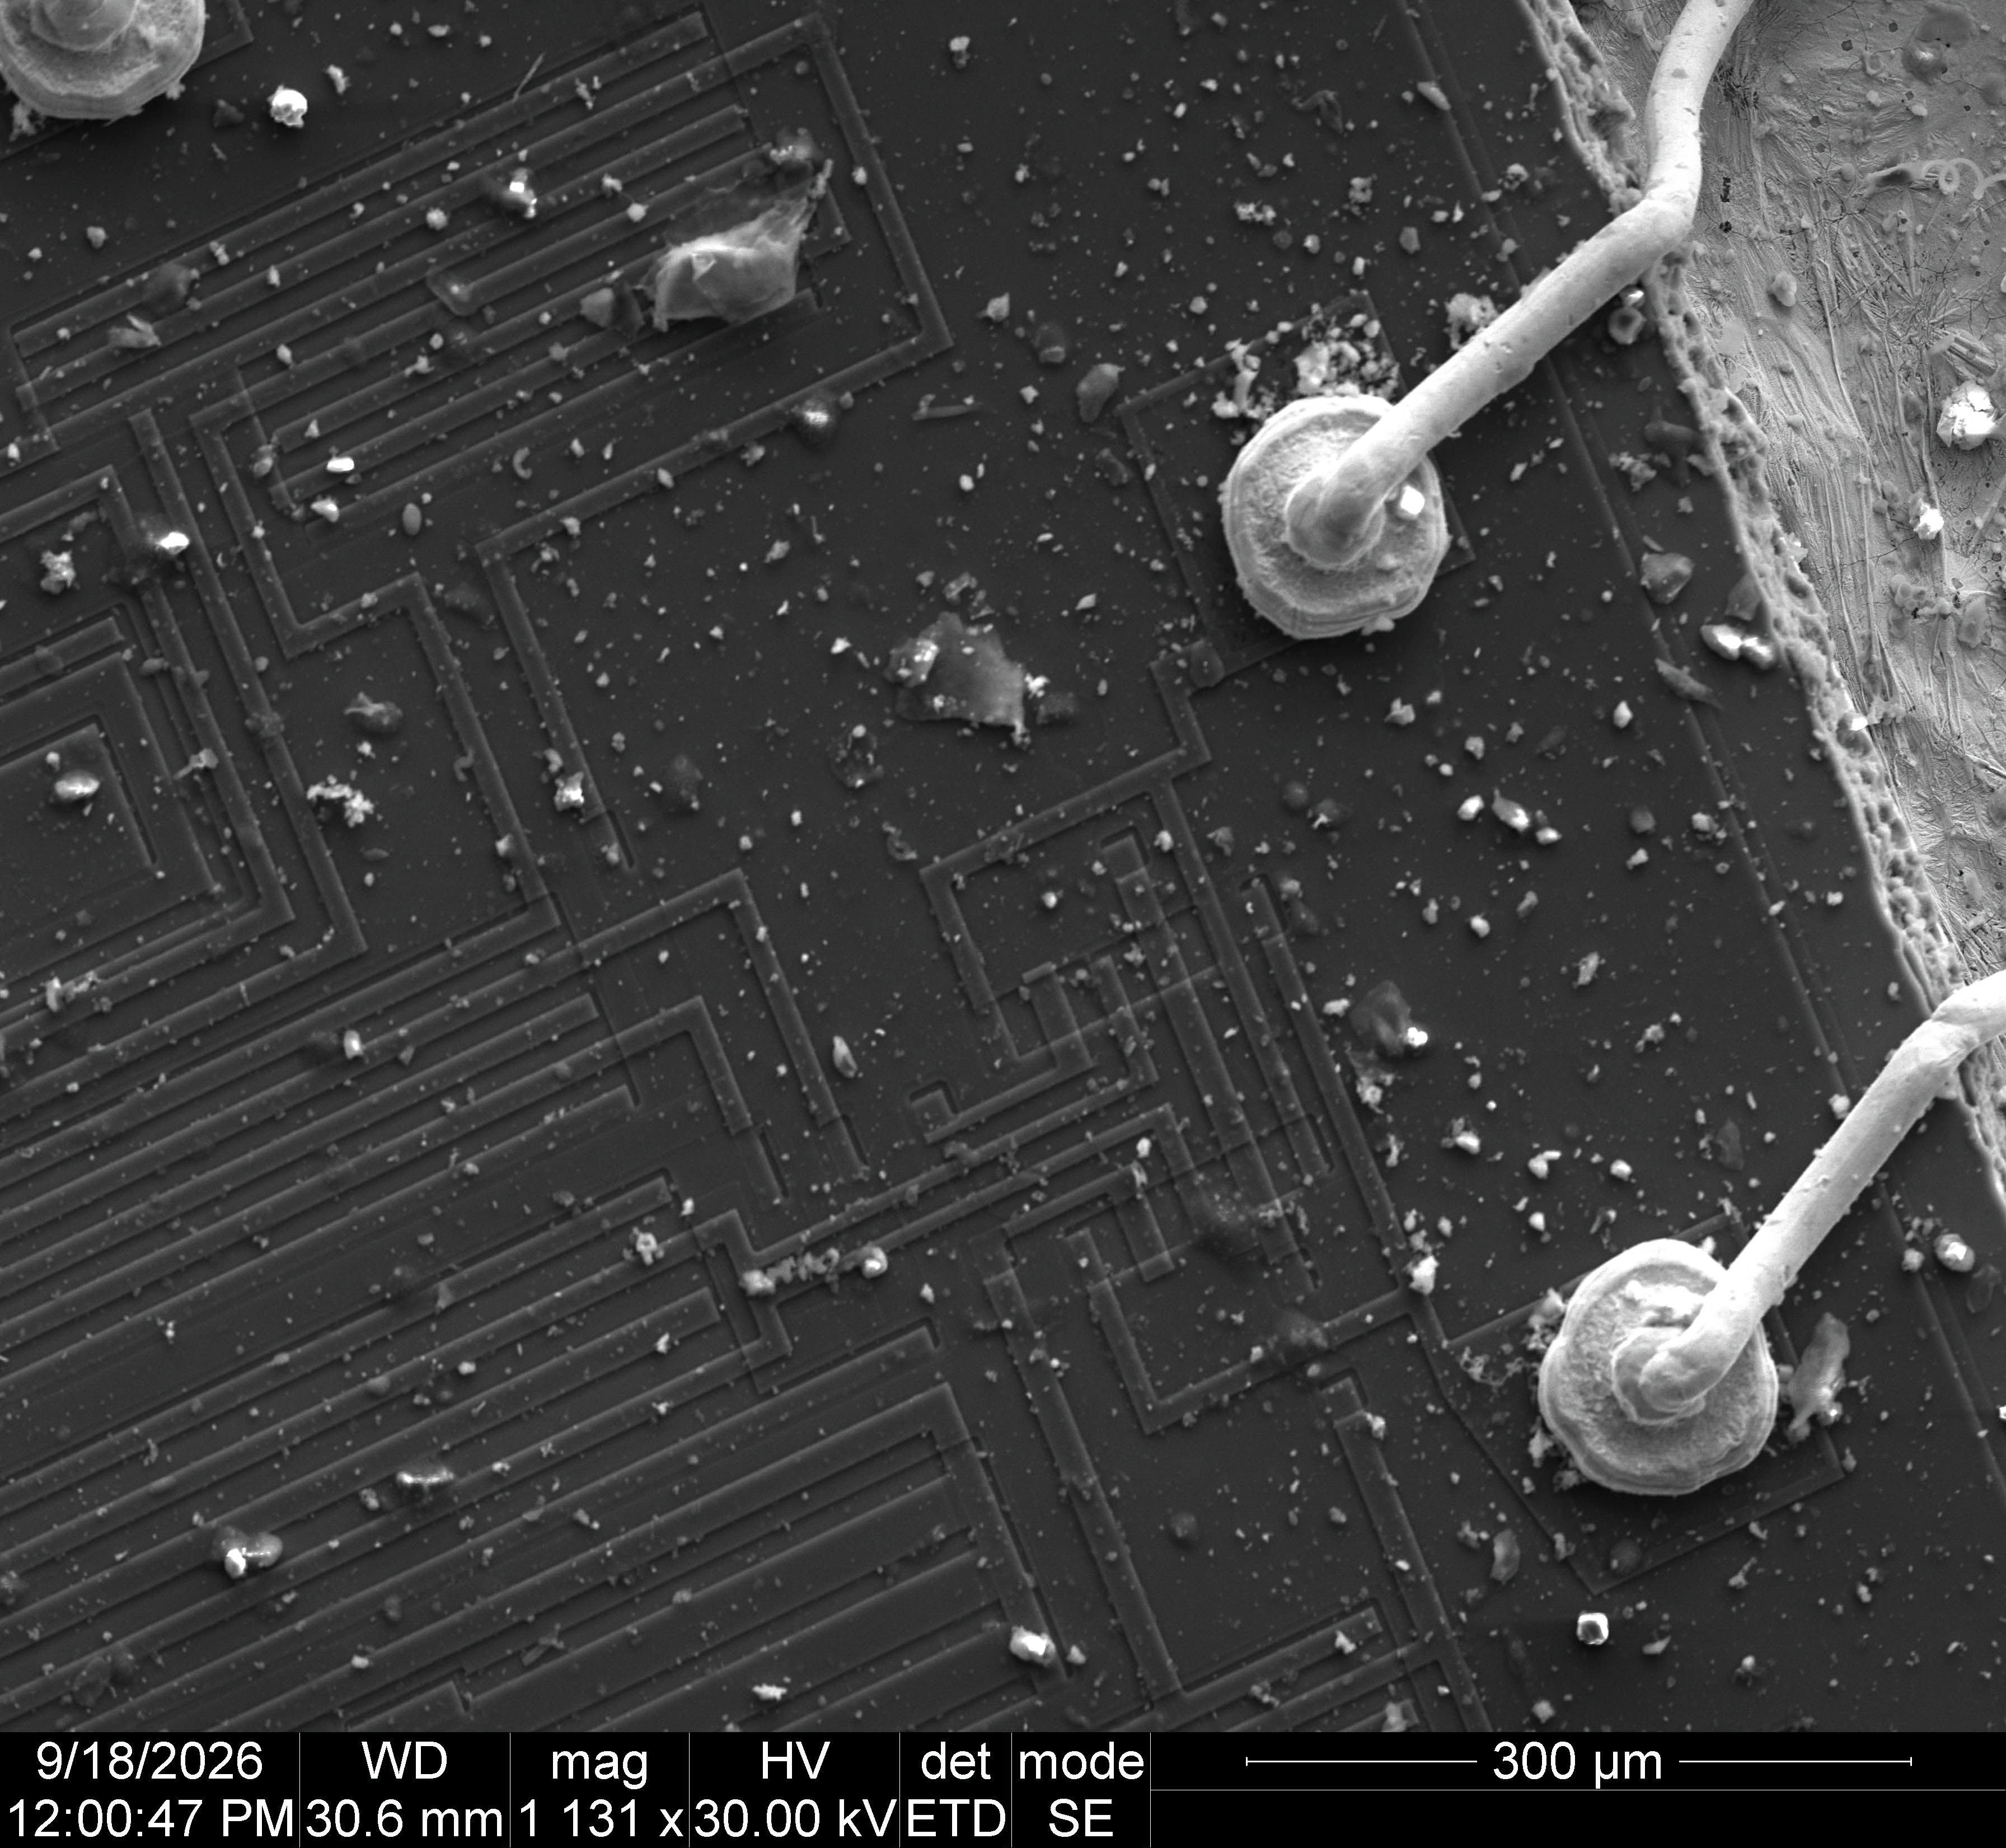
\includegraphics[width=\textwidth]{000.jpg}
        \caption{Изображение фрагмента микросхемы, Увеличение $1131\times$}
        \label{fig:chip_se}
    \end{minipage}
    \hfill
    \begin{minipage}{0.48\textwidth}
        \centering
        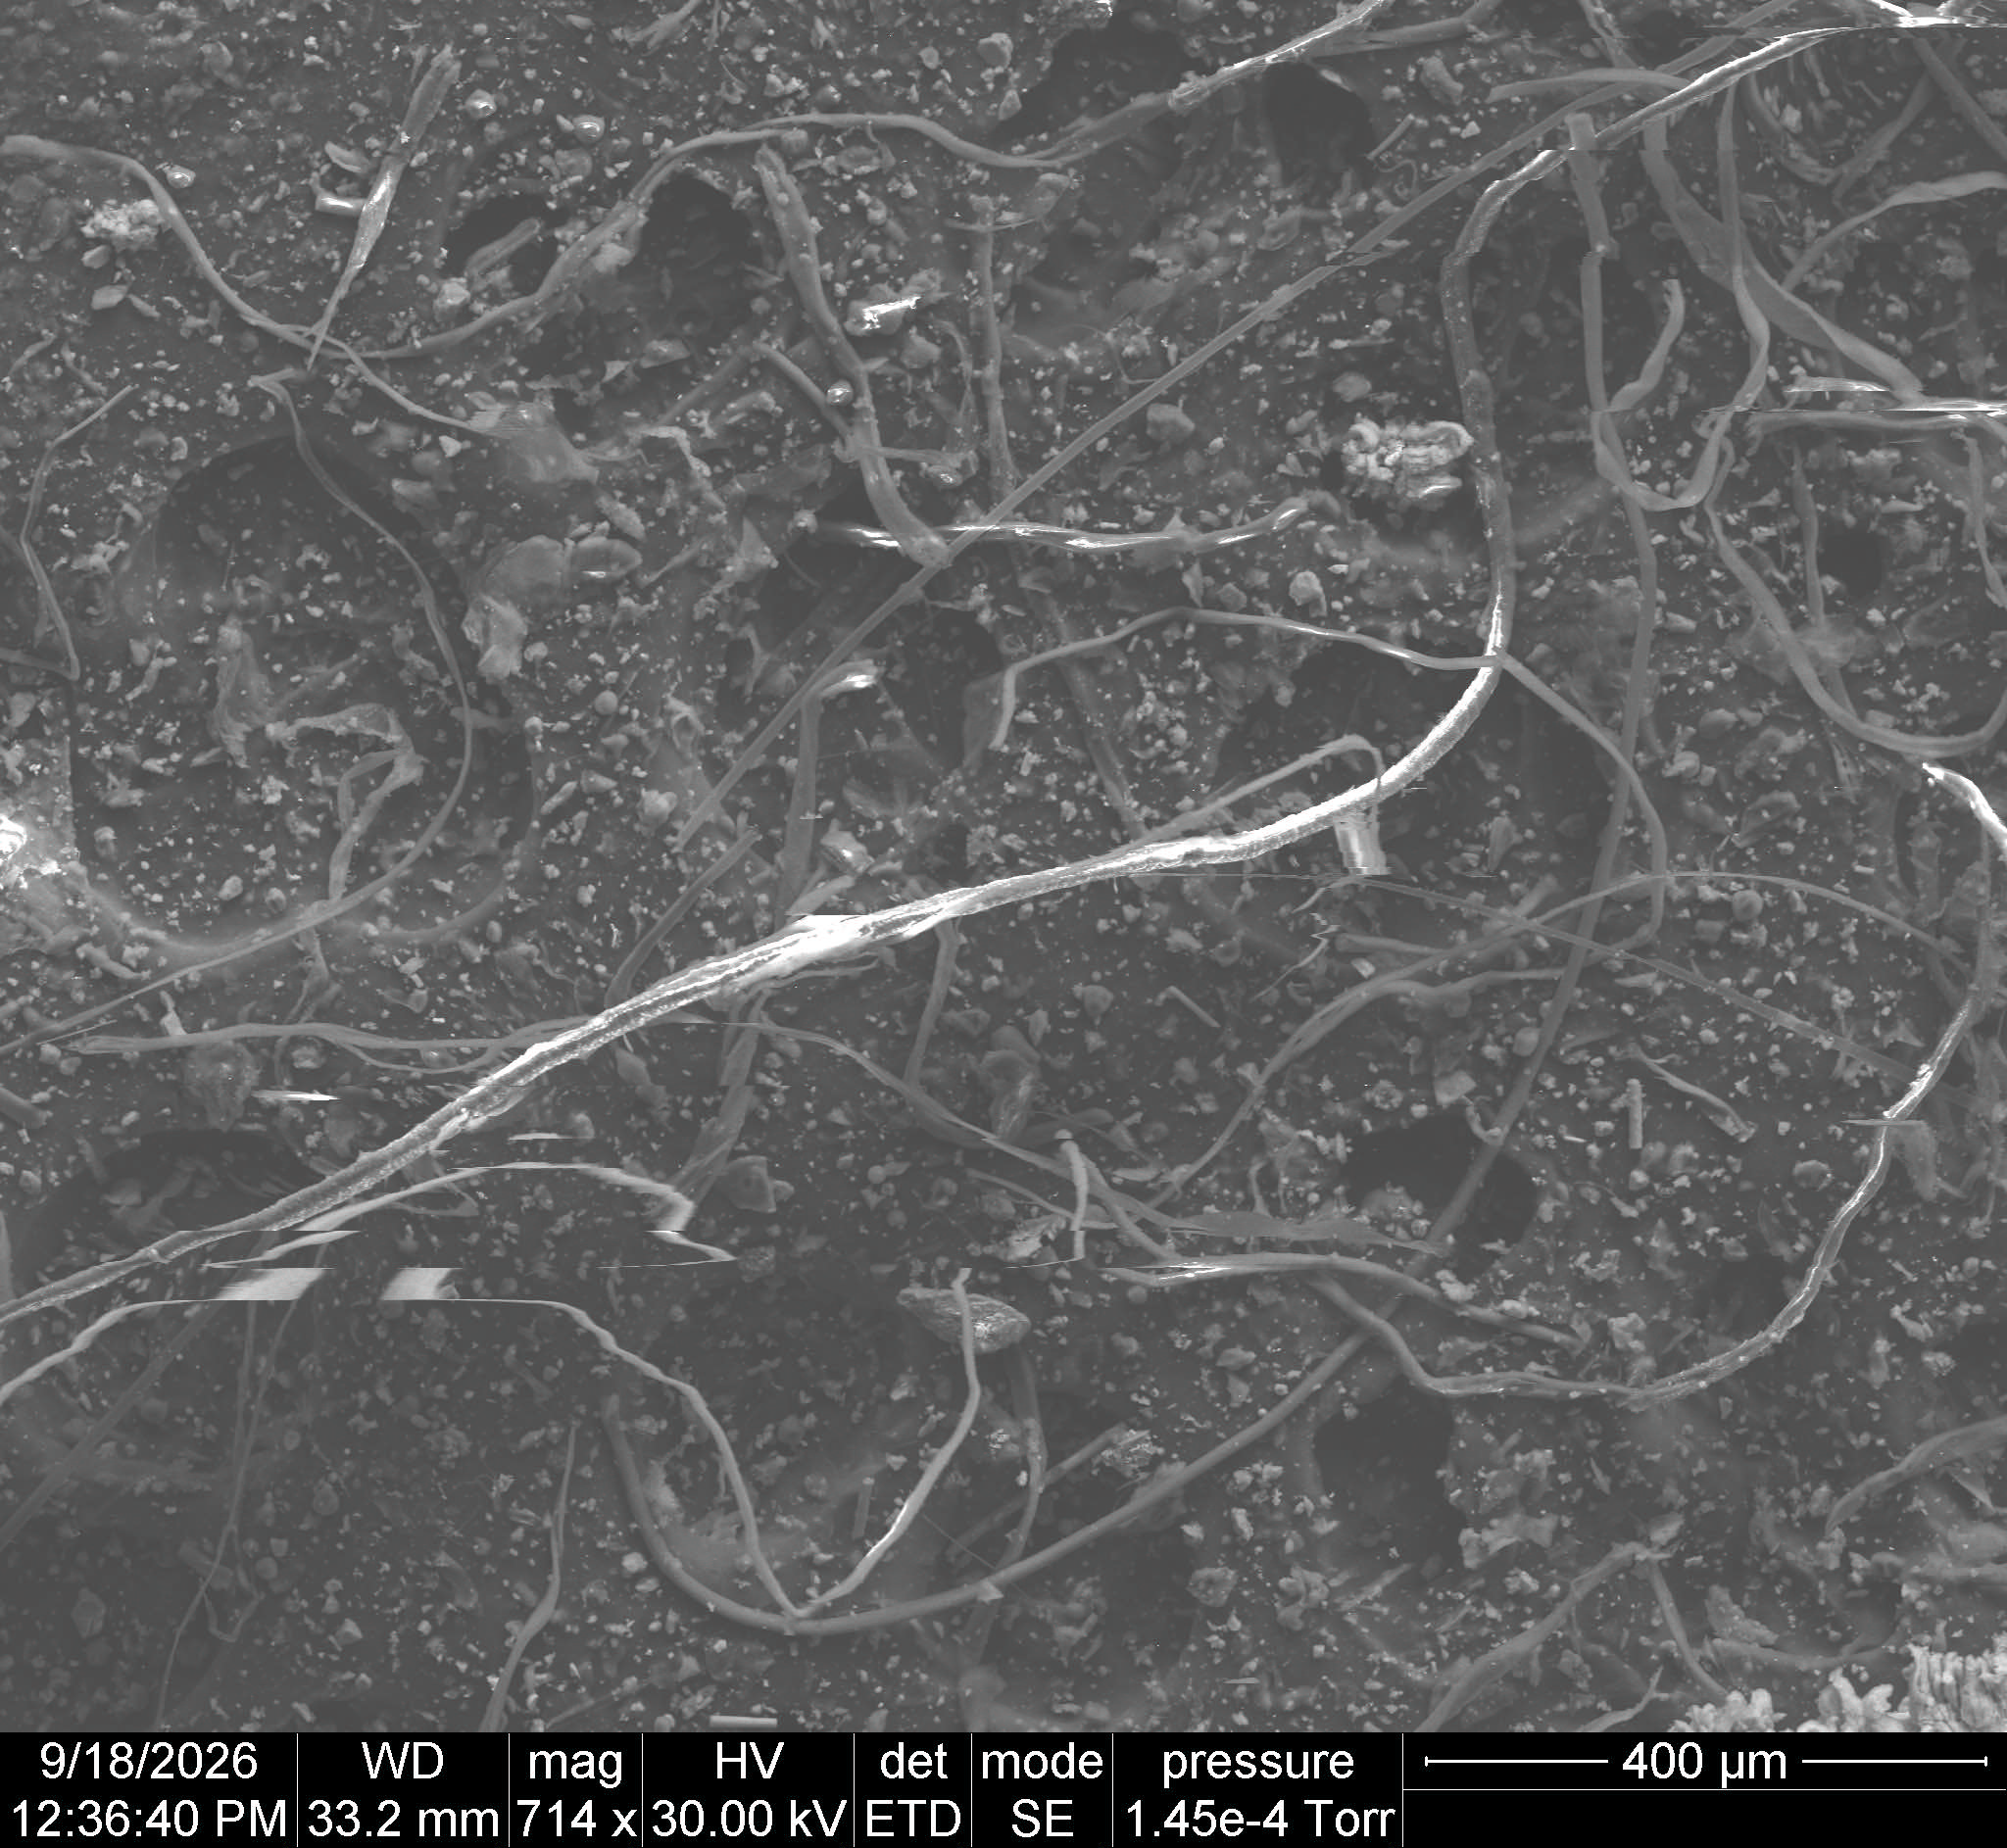
\includegraphics[width=\textwidth]{000_005.jpg}
        \caption{Изображение скотча, увеличение $714\times$}
        \label{fig:tape_se}
    \end{minipage}
\end{figure}

% На рис.~\ref{fig:chip_se} представлено изображение фрагмента микросхемы. Отчётливо видны тонкие металлические дорожки, образующие характерный узор, контактные площадки и проволочные выводы (wire bonds), соединяющие кристалл с корпусом. Поверхность микросхемы покрыта мелкими частицами --- вероятно, загрязнениями, попавшими на образец при подготовке.

% На рис.~\ref{fig:tape_se} показано изображение скотча --- диэлектрического полимерного материала. Поскольку скотч не проводит электрический ток, при облучении электронным пучком на его поверхности накапливается заряд, что приводит к искажениям изображения. Для борьбы с этим эффектом съёмка проводилась в режиме пониженного давления ($1{,}45\cdot10^{-4}$~Торр): молекулы остаточного газа в камере ионизируются электронным пучком, и положительные ионы нейтрализуют отрицательный заряд на поверхности образца. На изображении видна волокнистая структура полимерной плёнки, поры и отдельные частицы.

\subsubsection*{Изображение крыла бабочки}

Для изучения морфологии биологических образцов было получено изображение чешуек крыла бабочки в режиме вторичных электронов (SE) при двух различных увеличениях.

\begin{figure}[h]
    \centering
    \begin{minipage}{0.48\textwidth}
        \centering
        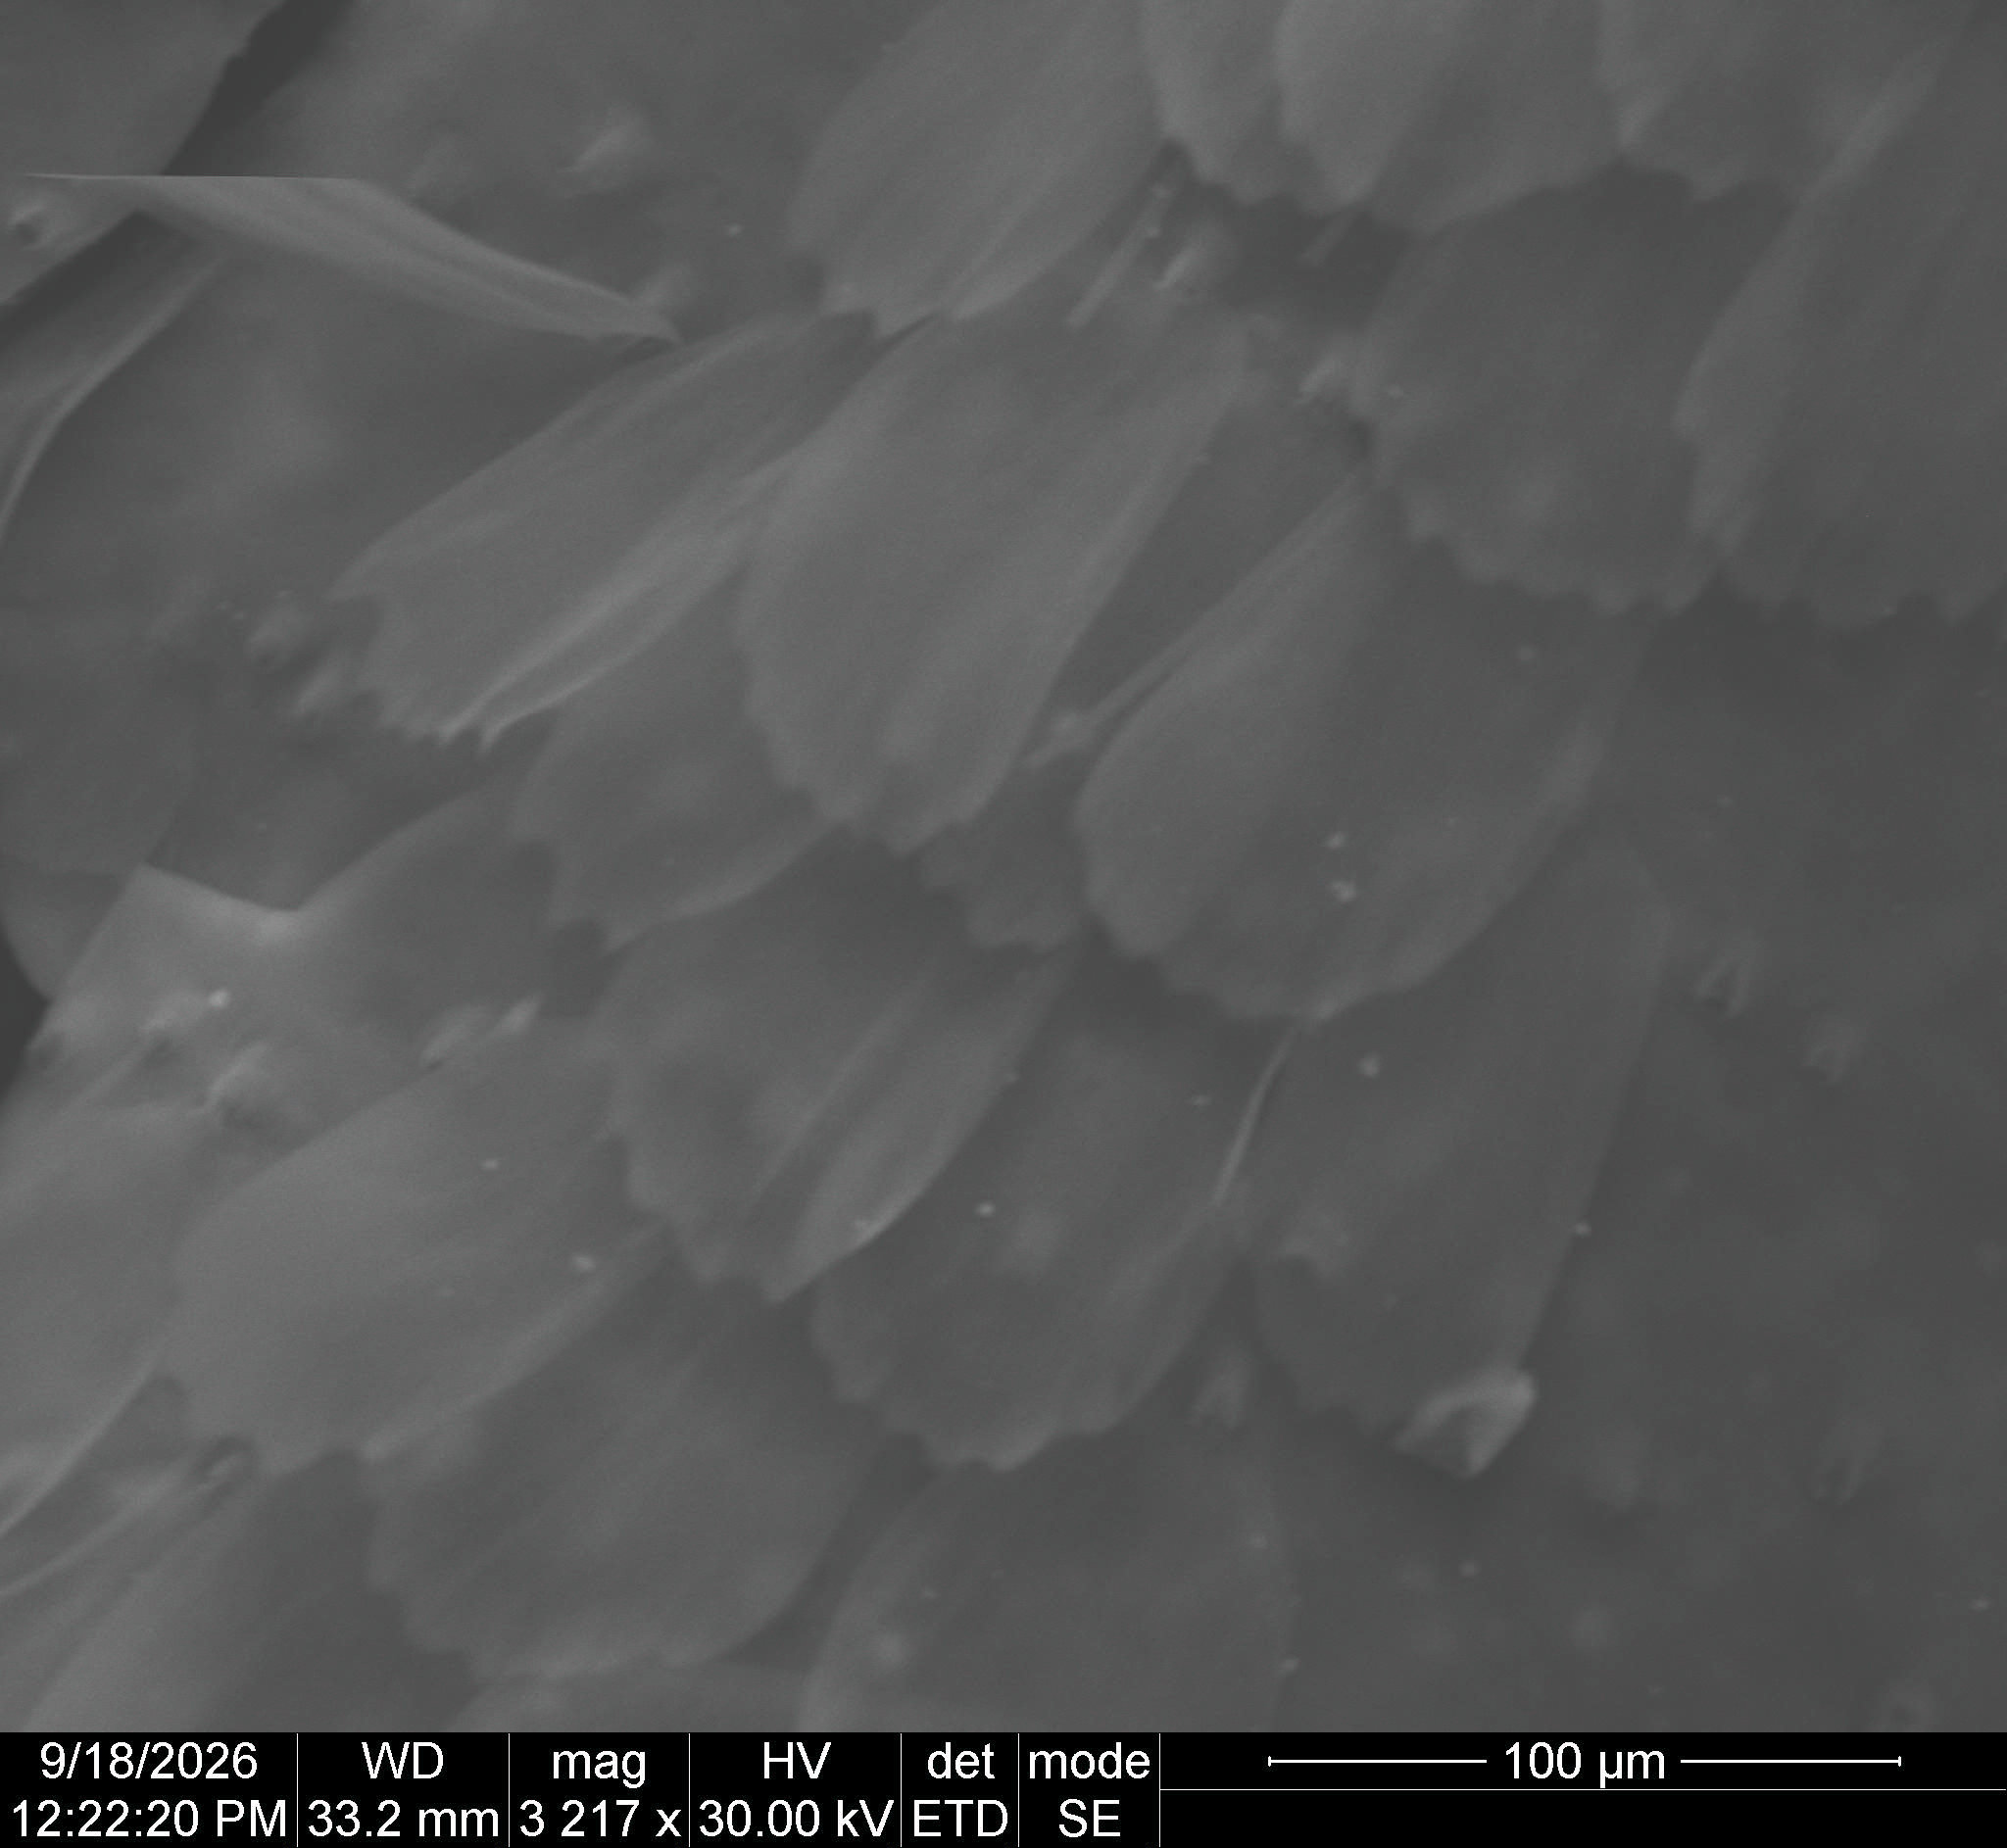
\includegraphics[width=\textwidth]{000_002.jpg}
        \caption{Изображение чешуек крыла бабочки при увеличении $3217\times$.}
        \label{fig:butterfly_low}
    \end{minipage}
    \hfill
    \begin{minipage}{0.48\textwidth}
        \centering
        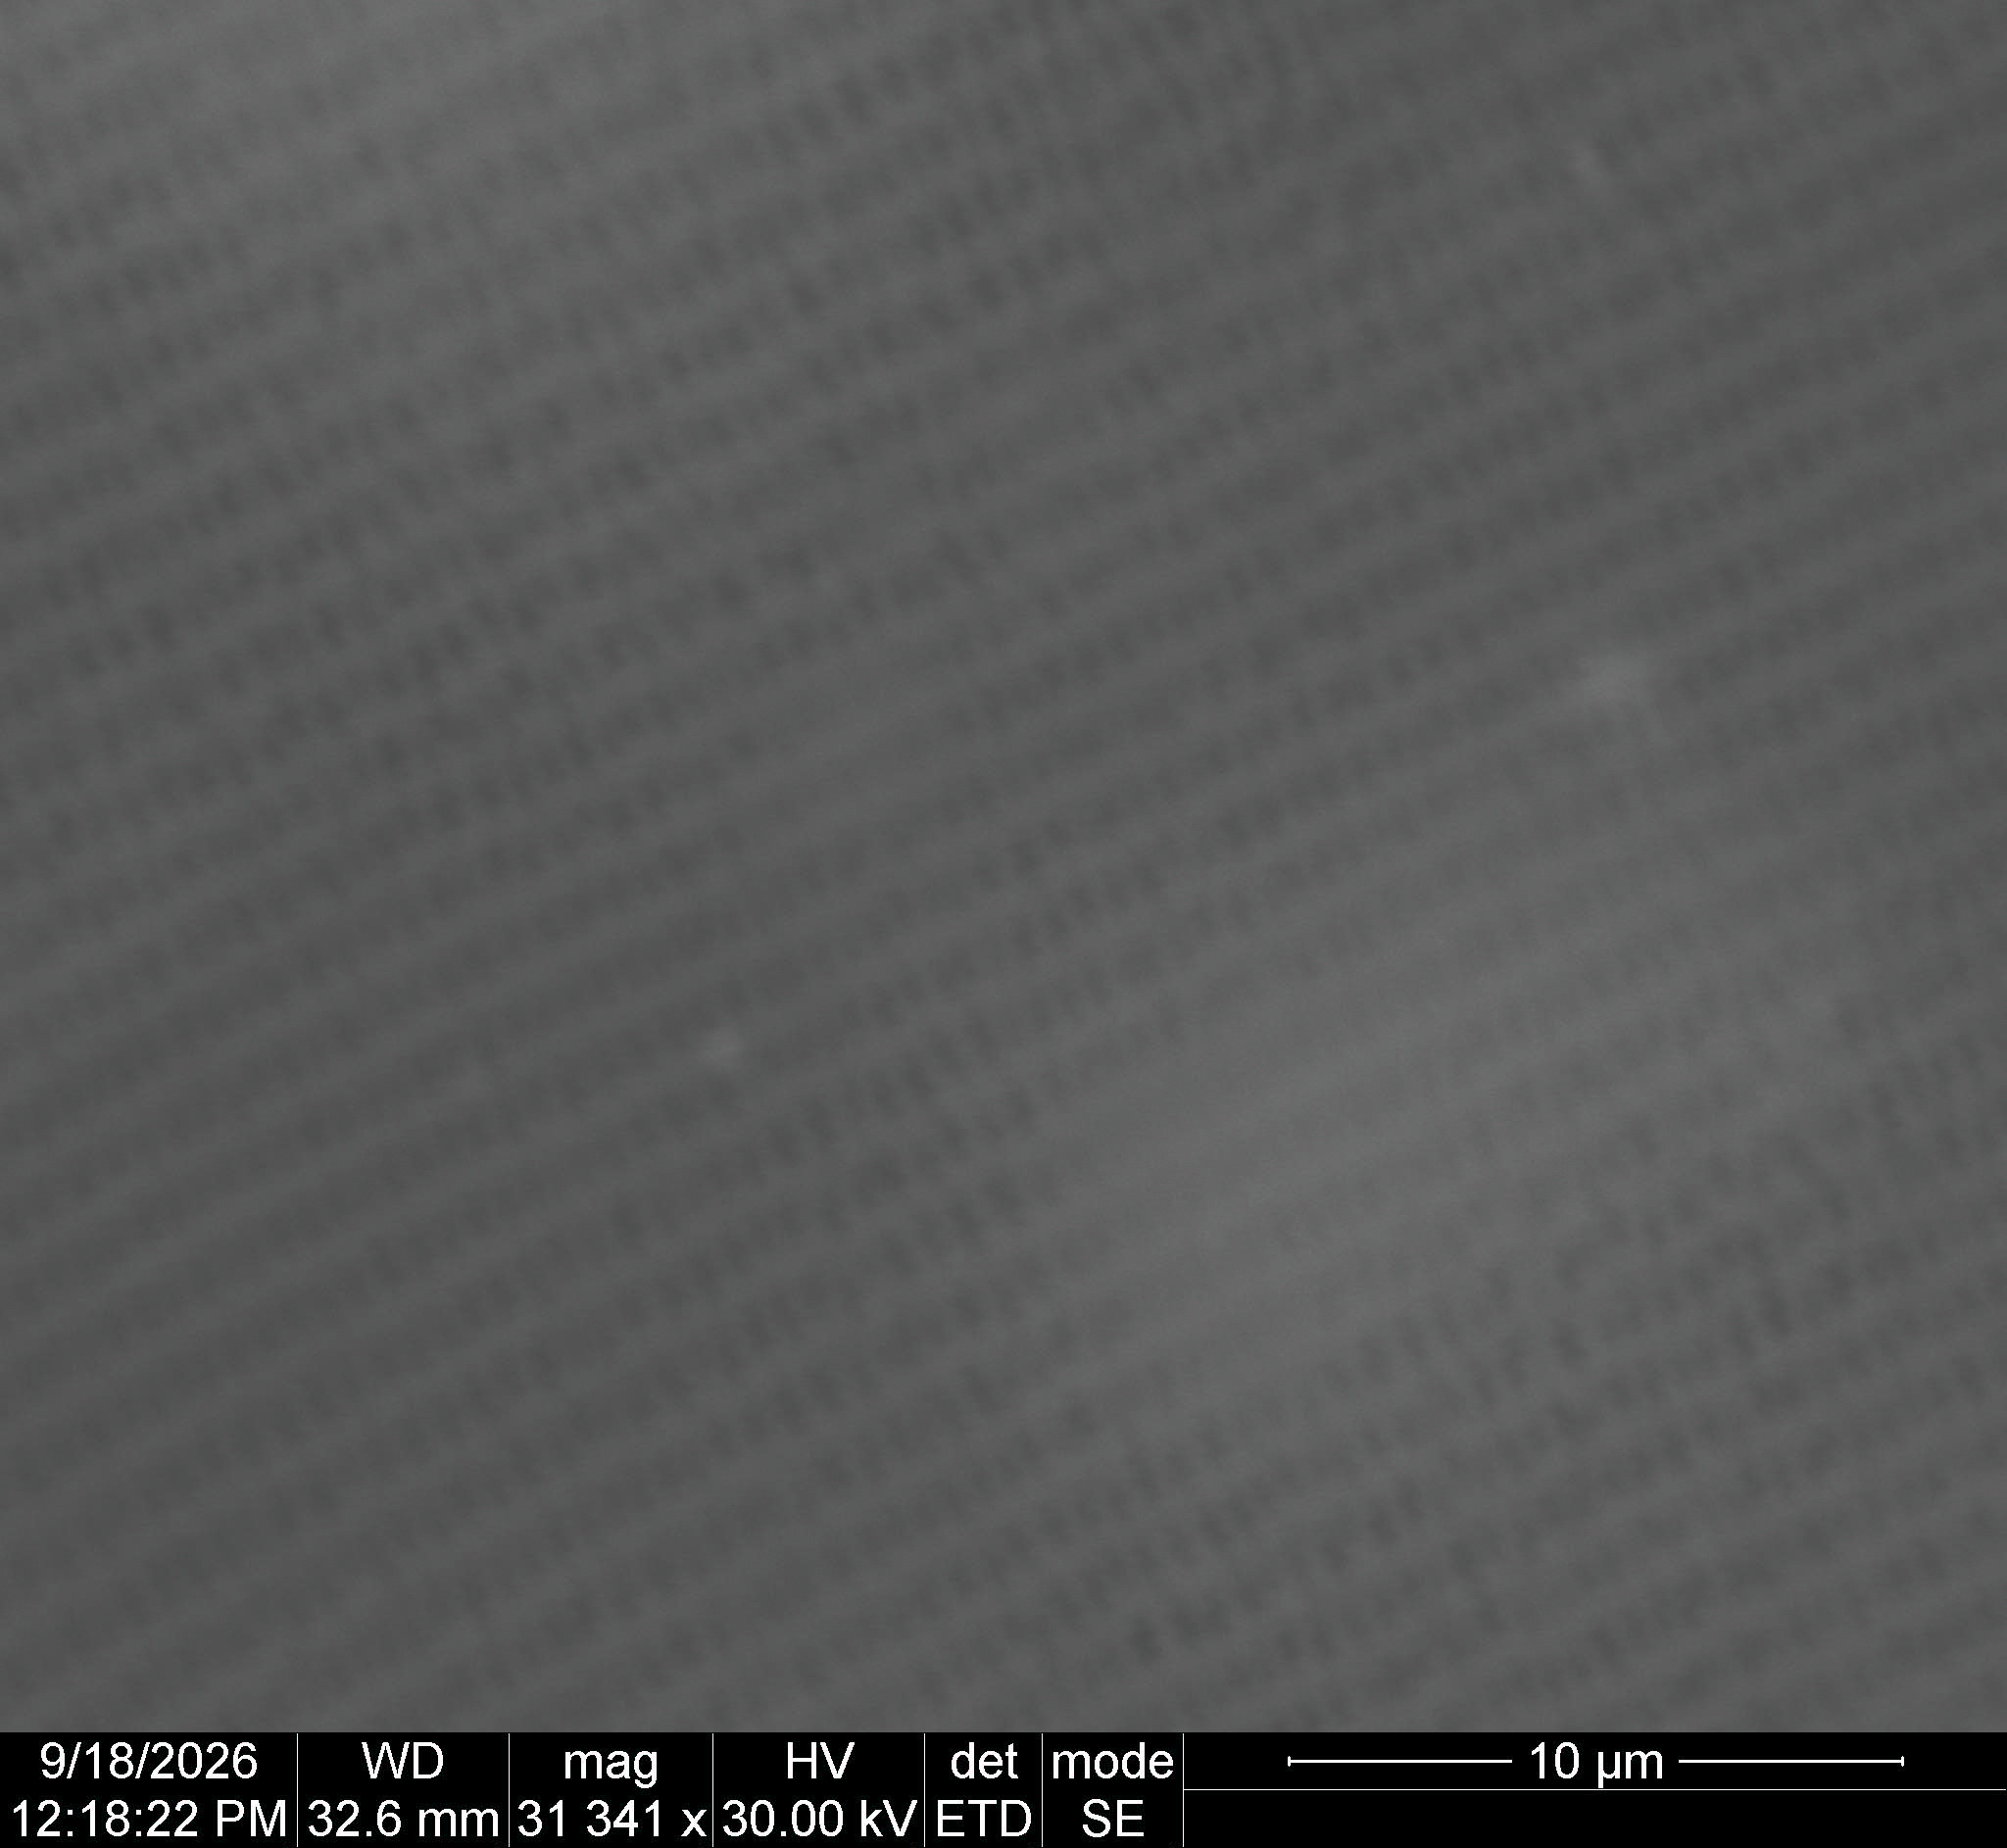
\includegraphics[width=\textwidth]{000_001.jpg}
        \caption{Изображение поверхности чешуйки при увеличении $31341\times$.}
        \label{fig:butterfly_high}
    \end{minipage}
\end{figure}

На рис.~\ref{fig:butterfly_low} при увеличении $3217\times$ отчётливо видна общая морфология чешуек крыла бабочки, их характерный размер составляет порядка $100$~мкм.

При большем увеличении $31341\times$ (рис.~\ref{fig:butterfly_high}) становится доступна тонкая структура поверхности чешуек. На изображении видна периодическая система продольных рёбер, идущих вдоль длинной оси чешуйки. Эти рёбра представляют собой наноструктуры с характерным периодом порядка сотен нанометров. Именно такая периодическая структура ответственна за структурную окраску крыльев бабочек --- явление, при котором цвет возникает не за счёт пигментов, а за счёт интерференции света на периодических наноструктурах.

% TODO: измерить период бороздок на изображении с высоким увеличением
% и сравнить с литературными данными





\subsubsection*{Сравнение режимов формирования изображения}

Для изучения различных типов контраста были получены изображения одного и того же участка образца в трёх режимах: регистрации вторичных электронов (SE), упругоотражённых электронов с суммированием сигналов сегментов (BSE, режим A+B) и с вычитанием сигналов (BSE, режим A-B).

\begin{figure}[h]
    \centering
    \begin{minipage}{0.32\textwidth}
        \centering
        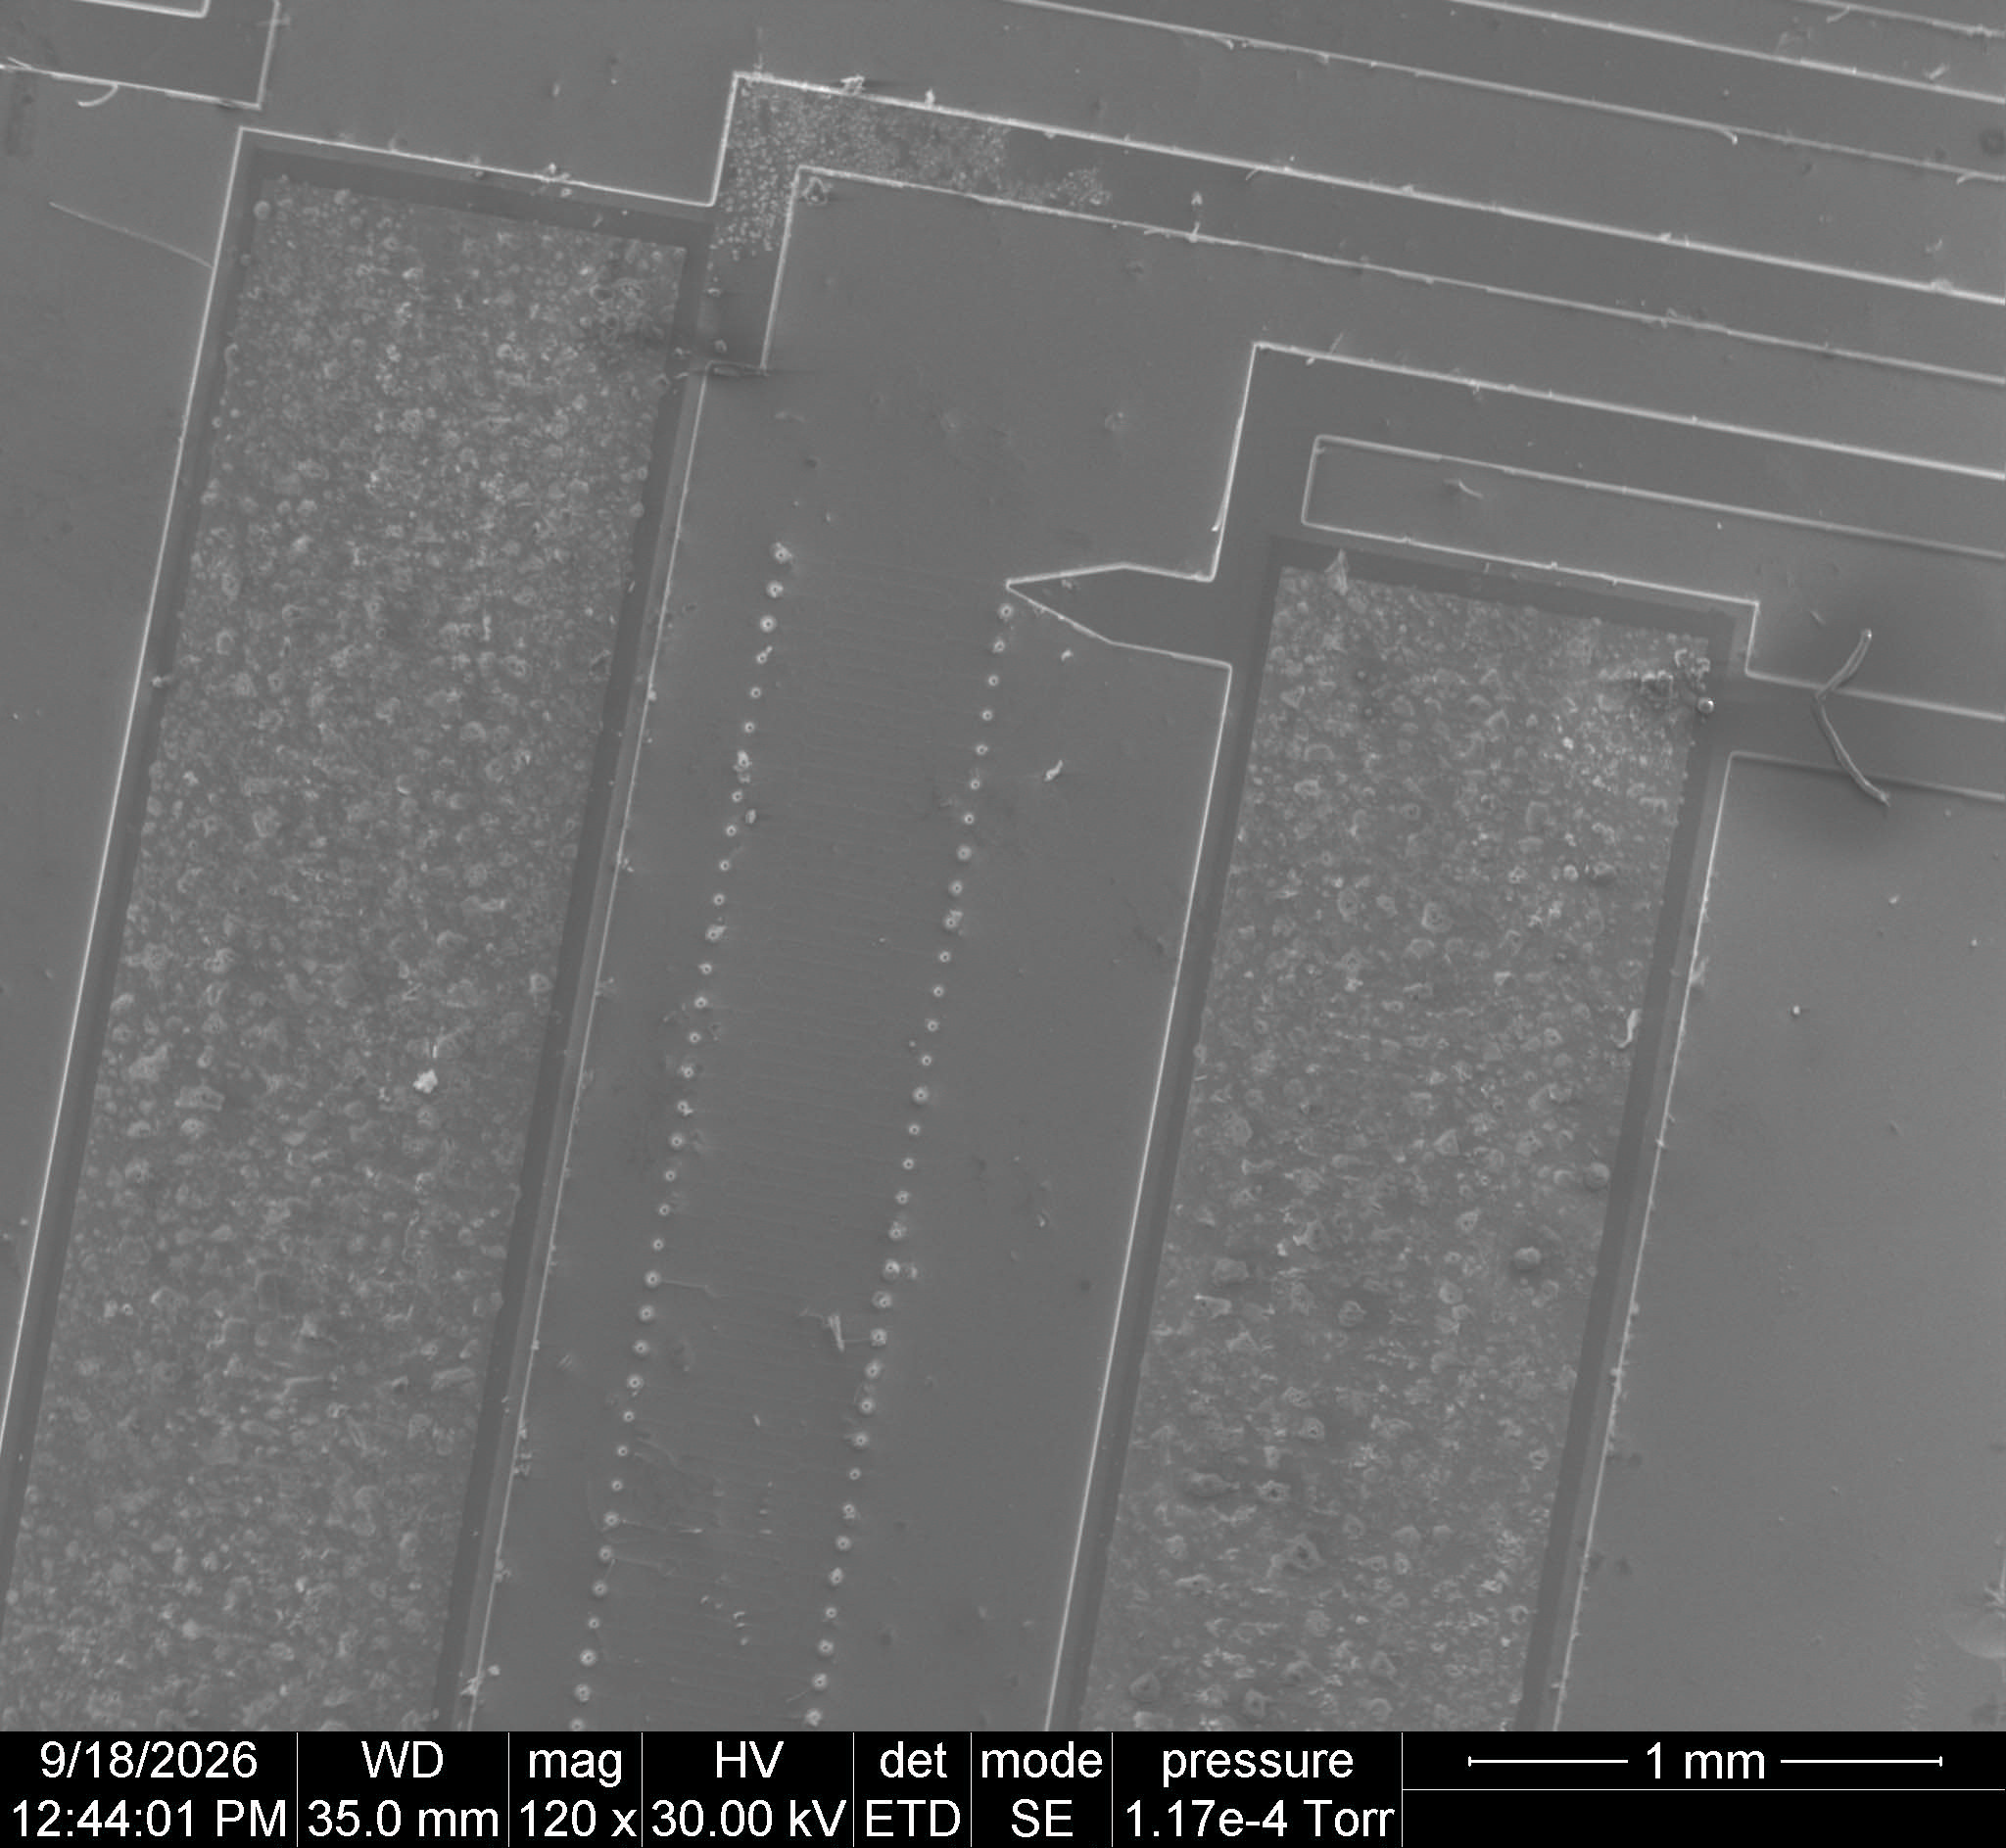
\includegraphics[width=\textwidth]{000_006.jpg}
        \caption{Режим SE (вторичные электроны).}
        \label{fig:se_mode}
    \end{minipage}
    \hfill
    \begin{minipage}{0.32\textwidth}
        \centering
        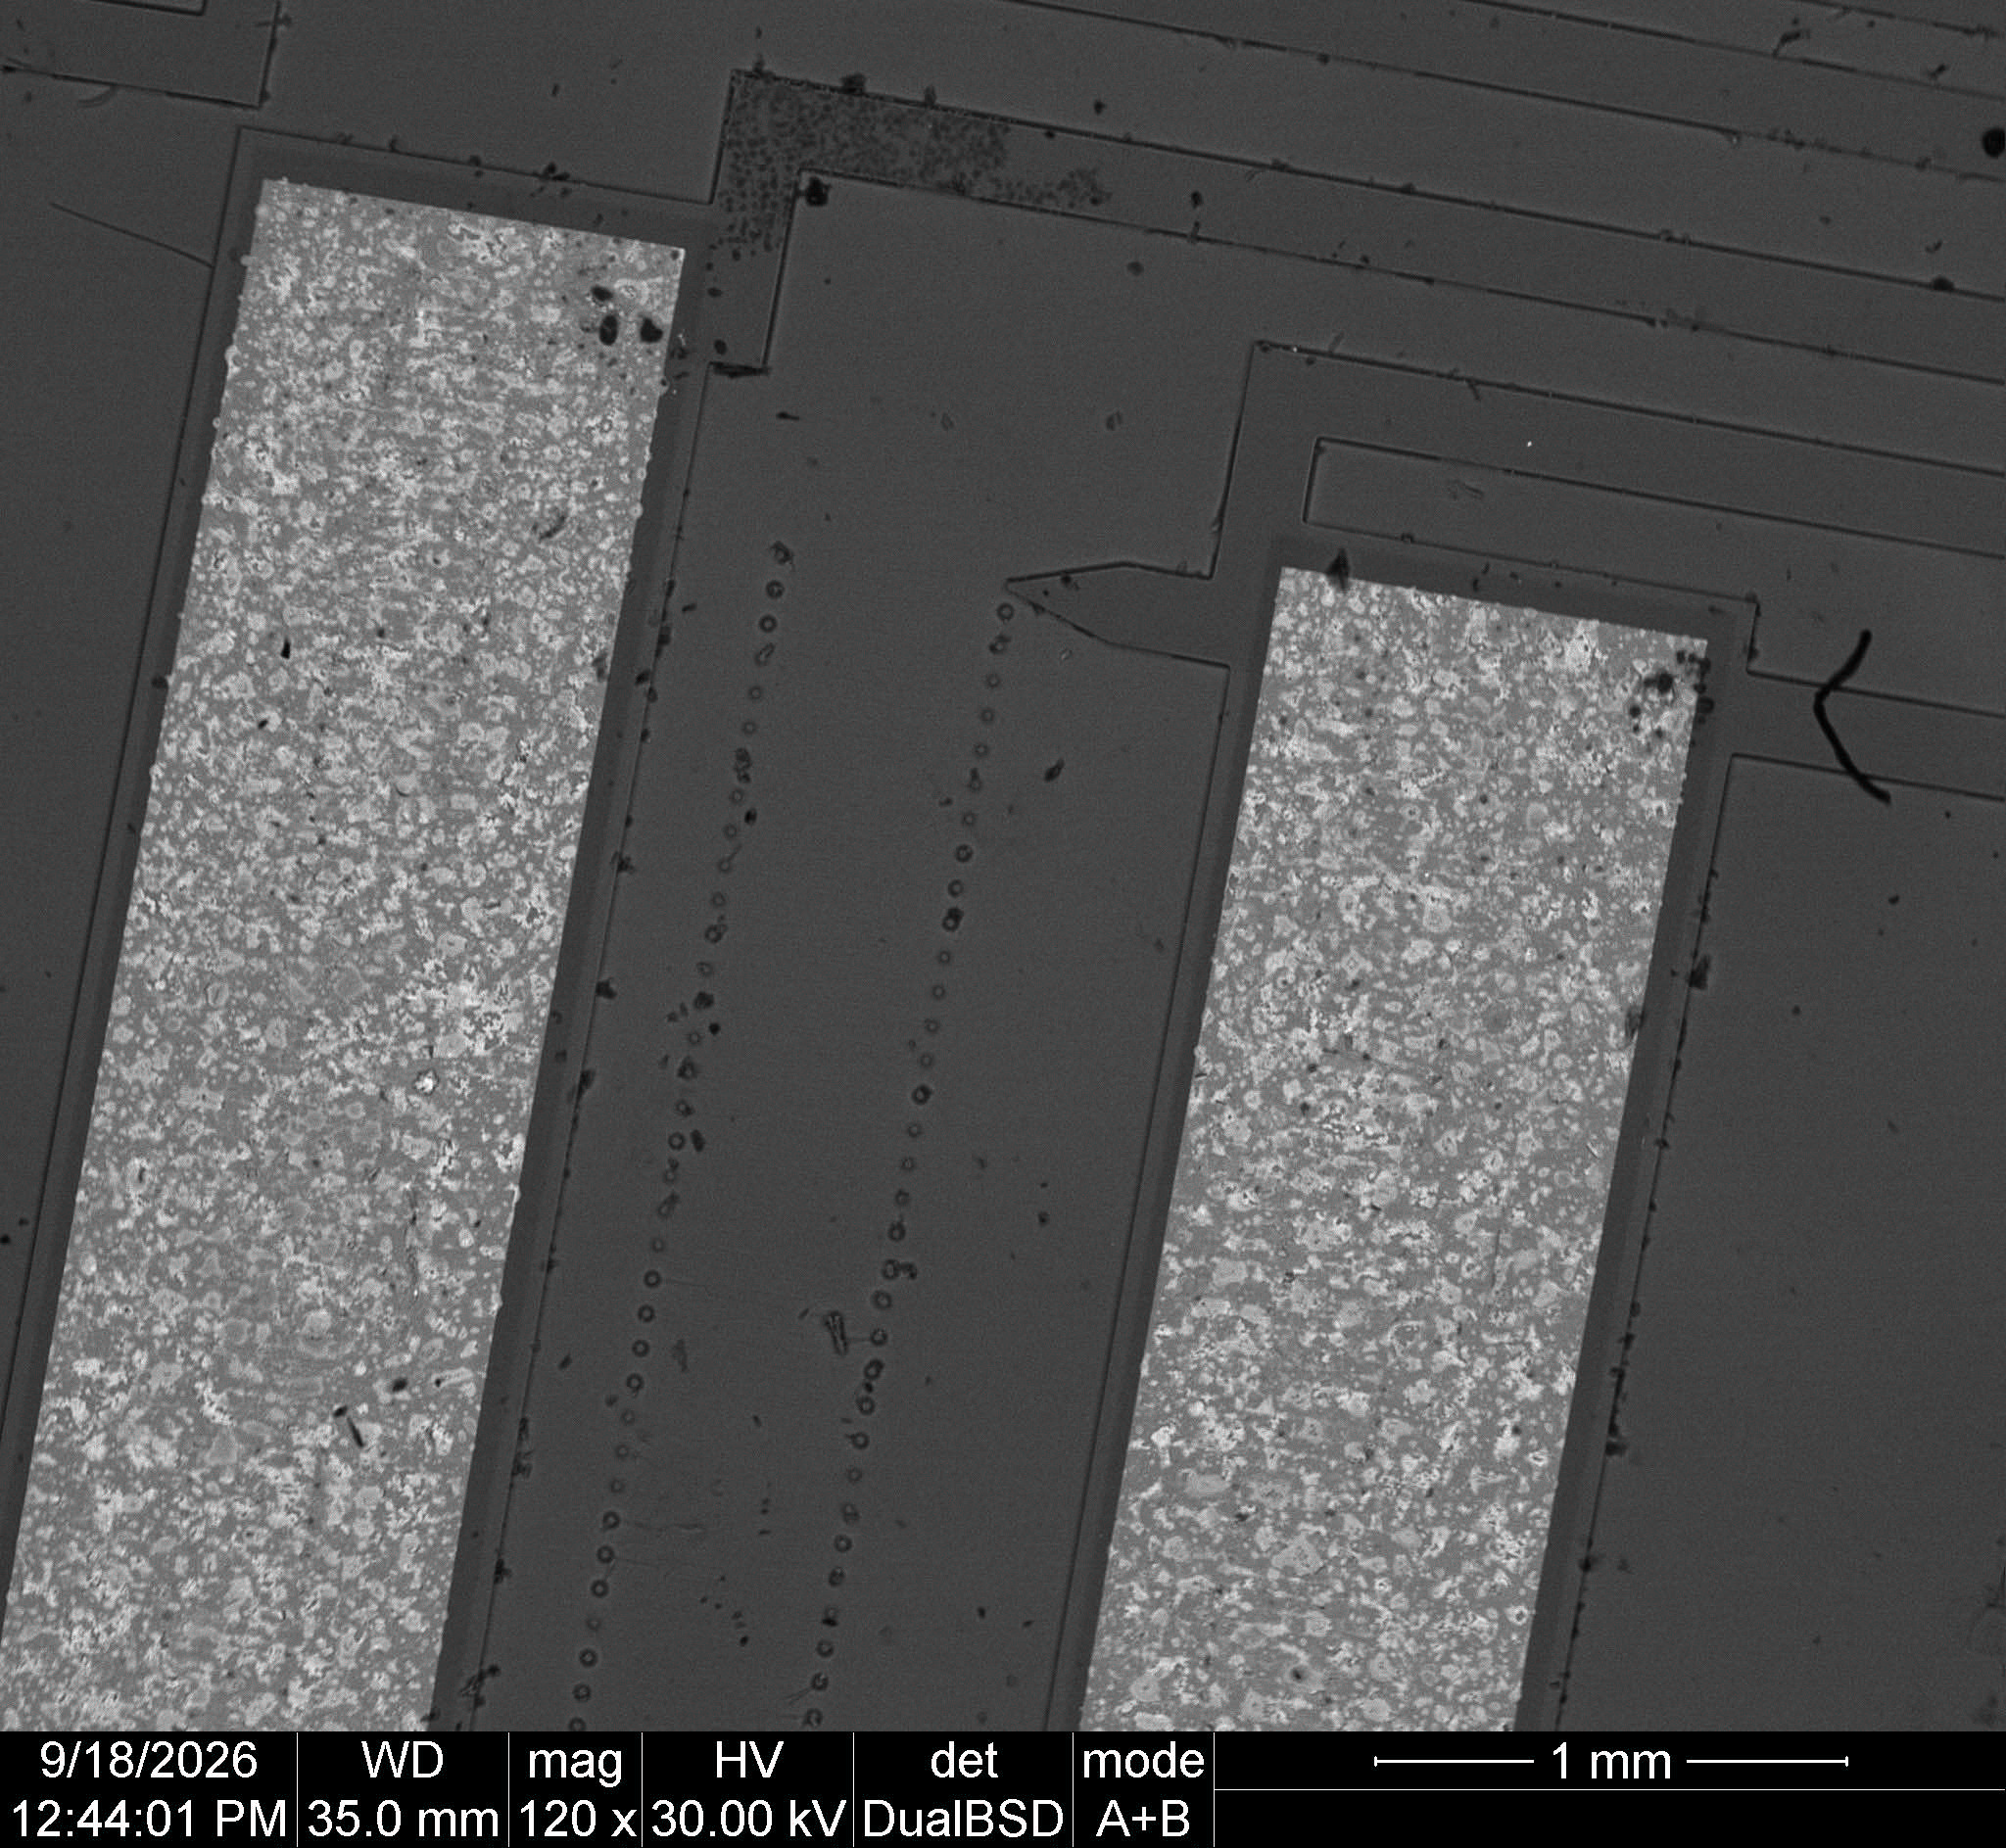
\includegraphics[width=\textwidth]{001_018.jpg}
        \caption{Режим BSE A+B (суммарный сигнал).}
        \label{fig:bse_sum}
    \end{minipage}
    \hfill
    \begin{minipage}{0.32\textwidth}
        \centering
        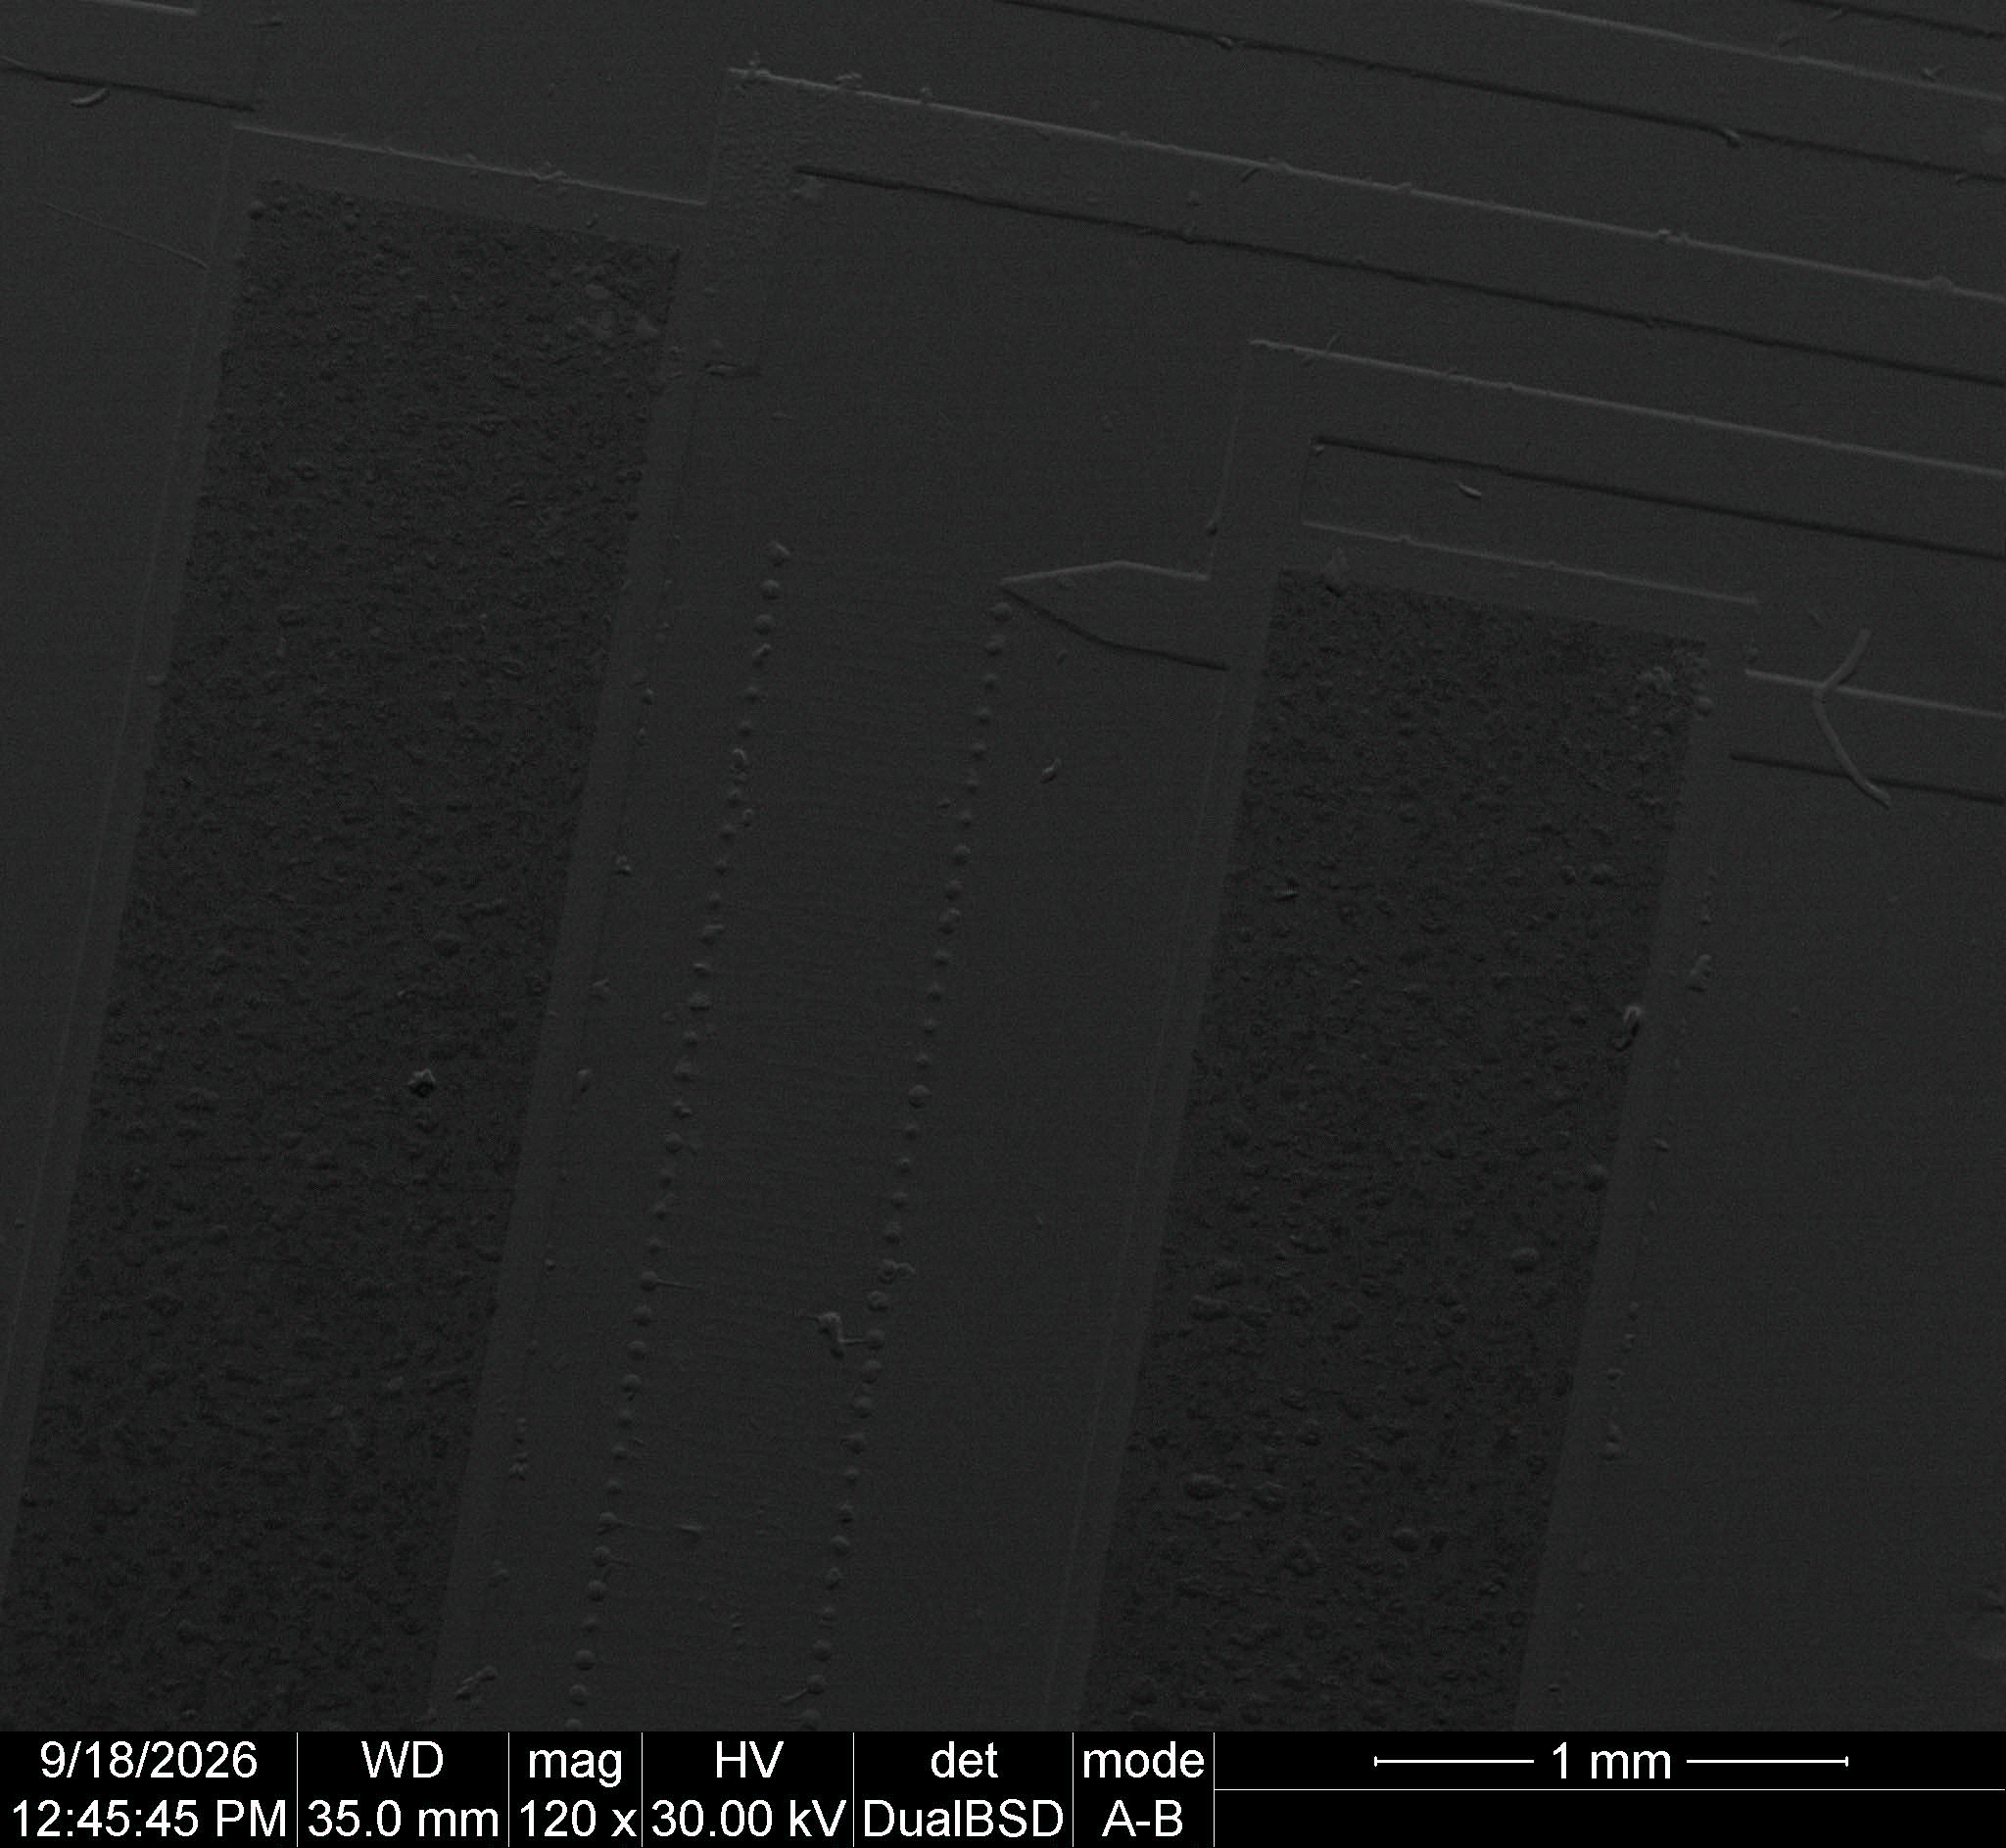
\includegraphics[width=\textwidth]{001_019.jpg}
        \caption{Режим BSE A-B (разностный сигнал).}
        \label{fig:bse_diff}
    \end{minipage}
\end{figure}

\textbf{Режим SE} (рис.~\ref{fig:se_mode}) обеспечивает классический топографический контраст. Вторичные электроны имеют низкую энергию ($0 < E < 50$~эВ) и выходят только с поверхностного слоя толщиной несколько нанометров. Интенсивность сигнала зависит от локального угла наклона поверхности: участки, повёрнутые к детектору, острые рёбра и выступы выглядят яркими, а углубления и тени --- тёмными. Этот режим наиболее нагляден для изучения морфологии поверхности.

\textbf{Режим BSE A+B} (рис.~\ref{fig:bse_sum}) реализует элементный (Z) контраст. Упругоотражённые электроны обладают высокой энергией (близкой к $E_0$) и вылетают из более глубоких слоёв образца (глубина выхода может достигать микрометров). При суммировании сигналов с обоих сегментов детектора топографические эффекты компенсируются, и яркость определяется преимущественно средним атомным номером материала: области с тяжёлыми элементами выглядят светлее, с лёгкими --- темнее. Этот режим используется для фазового анализа и выявления включений с различным химическим составом.

\textbf{Режим BSE A-B} (рис.~\ref{fig:bse_diff}) демонстрирует усиленный топографический контраст на упругоотражённых электронах. При вычитании сигналов сегментов элементный контраст уничтожается, а топографическая составляющая усиливается: наклоны поверхности, повёрнутые к одному сегменту, выглядят ярко, а к другому --- тёмно. Горизонтальные участки становятся серыми. Этот режим создаёт эффект ``псевдо-3D'' и особенно эффективен для выявления мелких неровностей, трещин и границ зёрен.

% Таким образом, три режима предоставляют взаимодополняющую информацию: SE даёт общее представление о рельефе поверхности, BSE~A+B показывает распределение элементов по атомному номеру, а BSE~A-B подчёркивает тонкие детали топографии с эффектом объёмности.







\subsection*{Исследование диэлектрического образца}

% В качестве диэлектрического образца был исследован пенопластовый шарик. Диэлектрики в РЭМ представляют особый интерес, поскольку при облучении электронным пучком на их поверхности накапливается электрический заряд, что приводит к ряду характерных артефактов.

% \subsubsection*{Зарядка диэлектрика в электронном пучке}

При бомбардировке диэлектрического образца электронами зонда возникшие вторичные и отражённые электроны уносят с поверхности часть заряда, однако значительная доля первичных электронов остаётся в объёме образца. Поскольку диэлектрик не обладает достаточной проводимостью для отвода накопленного заряда, на его поверхности формируется локальный отрицательный заряд. Этот заряд создаёт электрическое поле, которое:
\begin{itemize}
    \item отклоняет первичный электронный пучок, искажая изображение;
    \item изменяет траектории вторичных электронов, что приводит к аномально ярким или тёмным областям;
    \item в предельном случае может действовать как электростатическое зеркало, отражая низкоэнергетичные электроны обратно в колонну микроскопа.
\end{itemize}

% \subsubsection*{Изображение пенопластового шарика}

На рис.~\ref{fig:foam_ball} представлено изображение пенопластового шарика, полученное в режиме SE.

\begin{figure}[h]
    \centering
    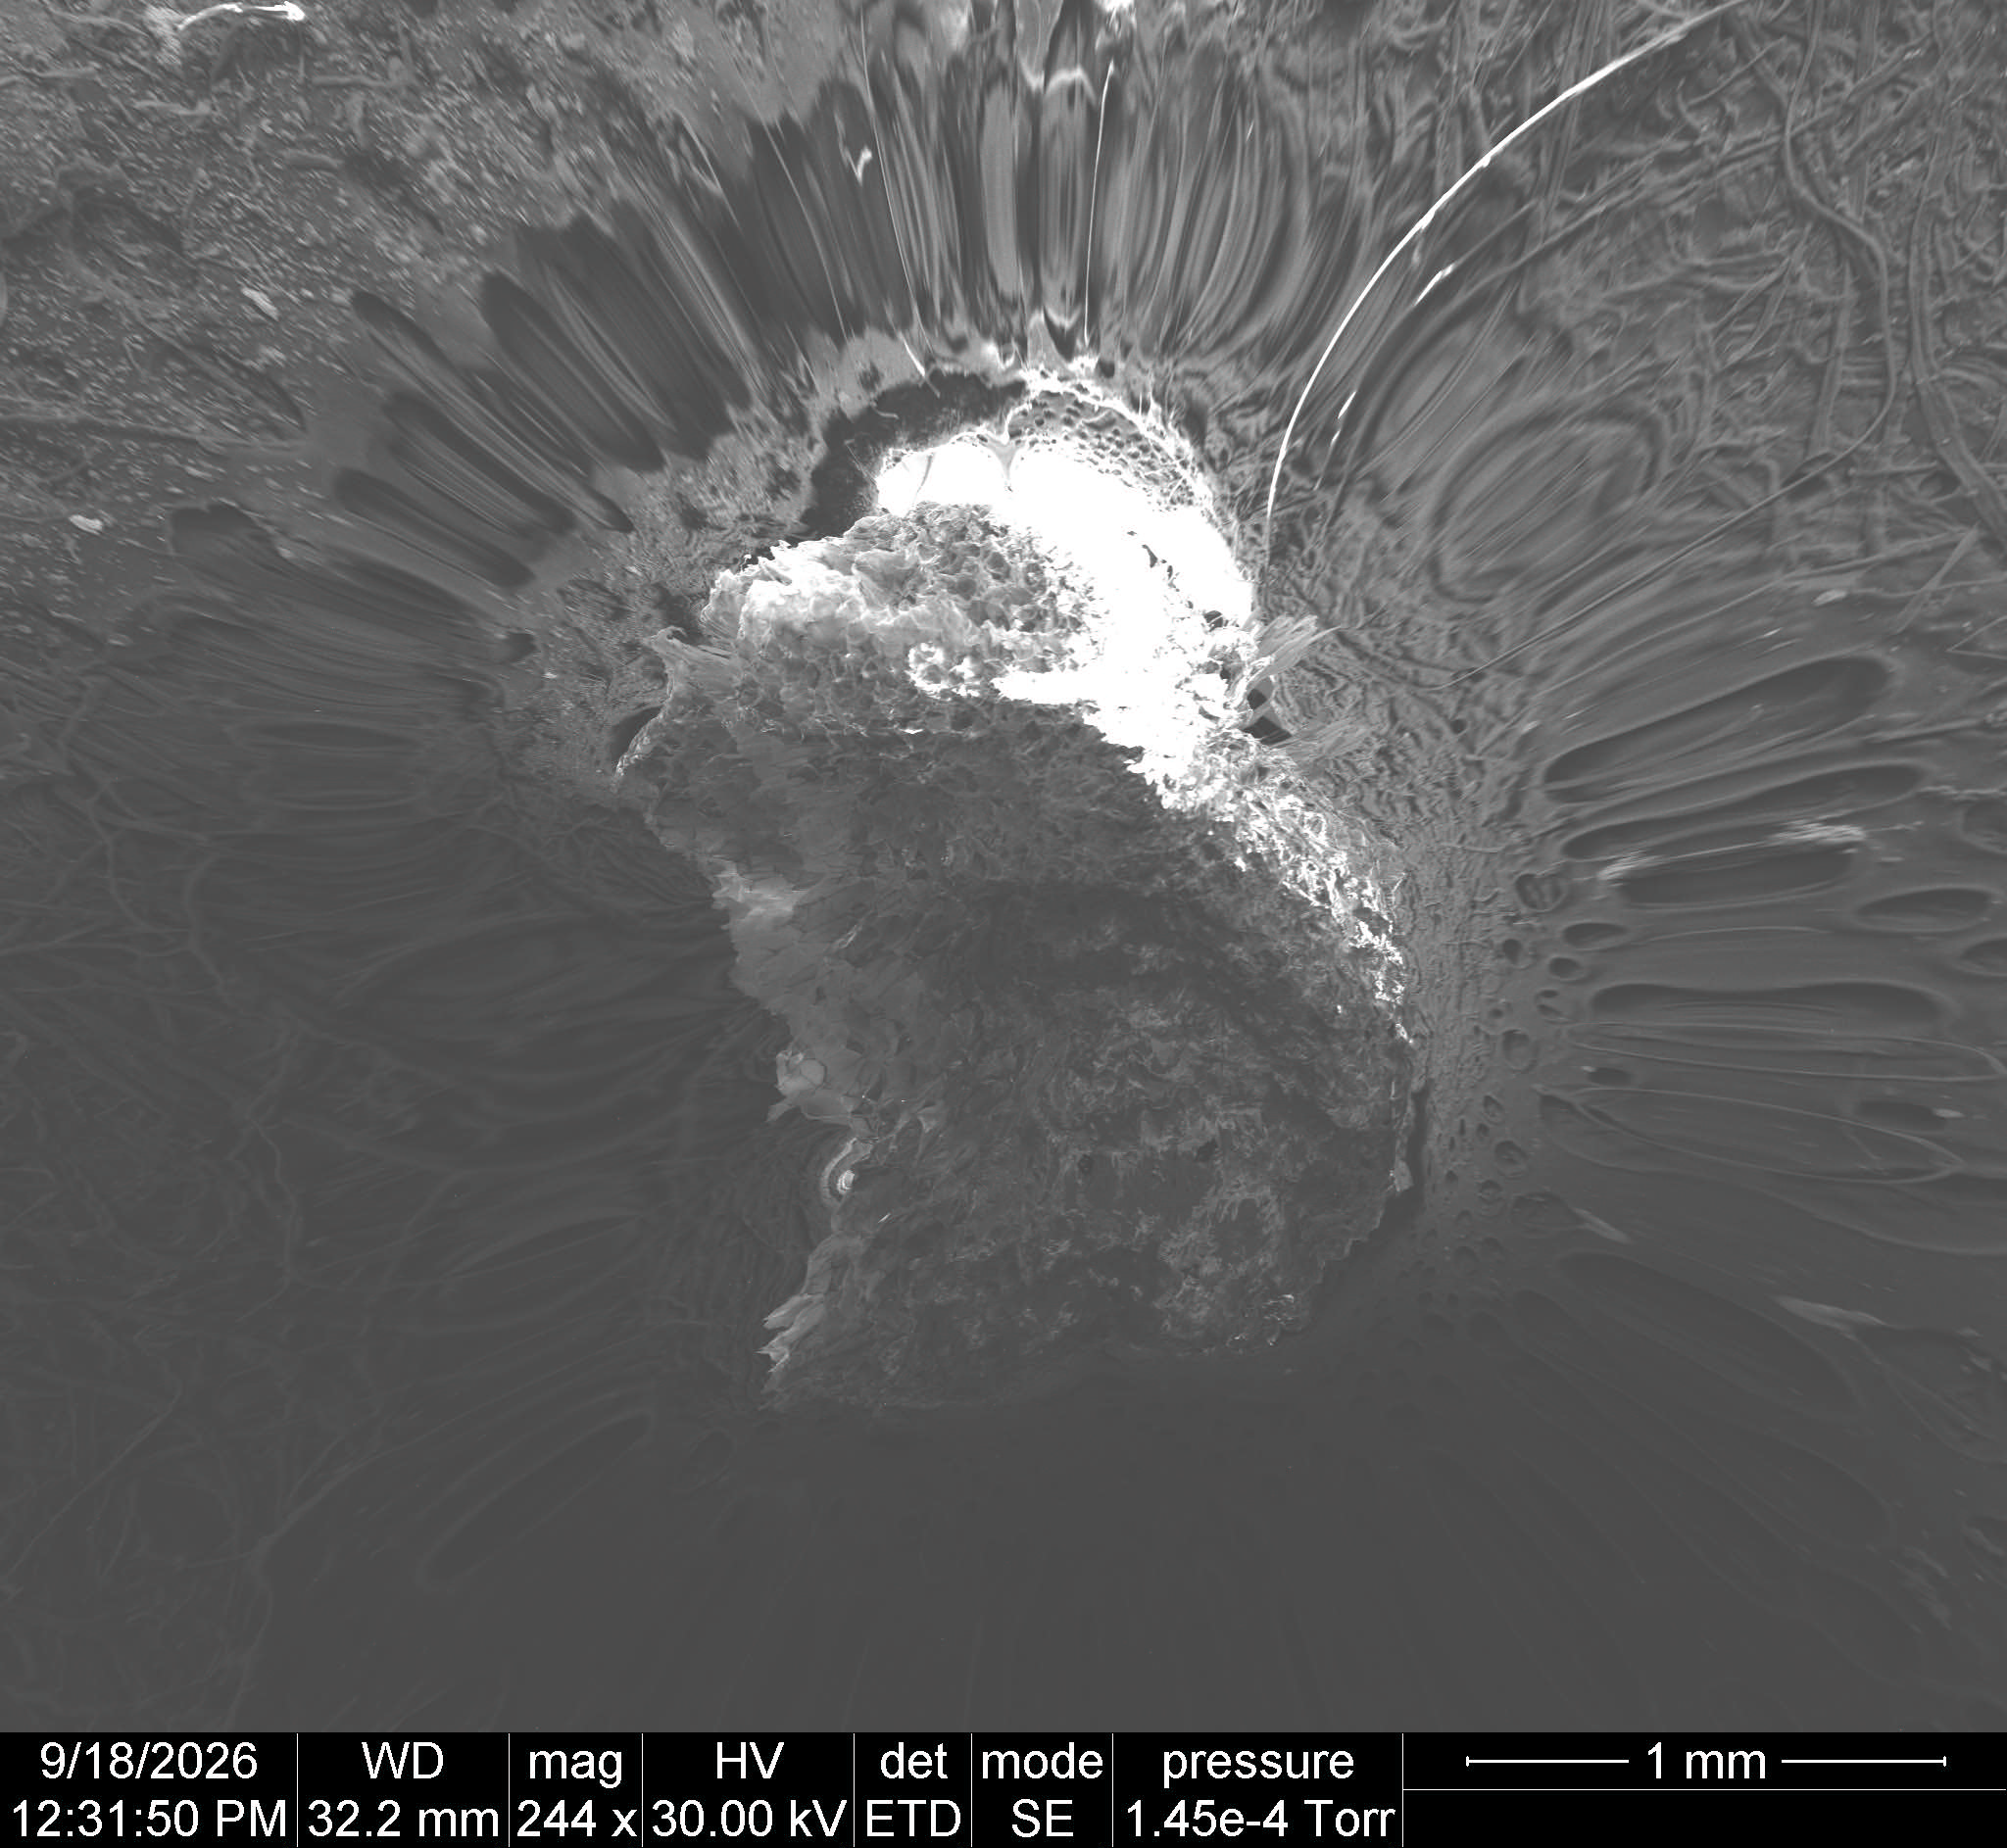
\includegraphics[width=0.5\textwidth]{000_003.jpg}
    \caption{Изображение пенопластового шарика.}
    \label{fig:foam_ball}
\end{figure}

% TODO: описать наблюдаемые артефакты зарядки на изображении шарика



\subsubsection*{Зеркальное изображение колонны микроскопа}

На рис.~\ref{fig:mirror} представлено так называемое «зеркальное» изображение, возникающее при облучении диэлектрического образца электронами с меньшей энергией. Накопленный на поверхности шарика отрицательный заряд действует как электростатическое зеркало: электроны зонда, не достигая поверхности образца, отражаются электрическим полем заряда и возвращаются в колонну микроскопа. В результате на детектор попадает сигнал, соответствующий не рельефу образца, а внутреннему устройству колонны.

\begin{figure}[h]
    \centering
    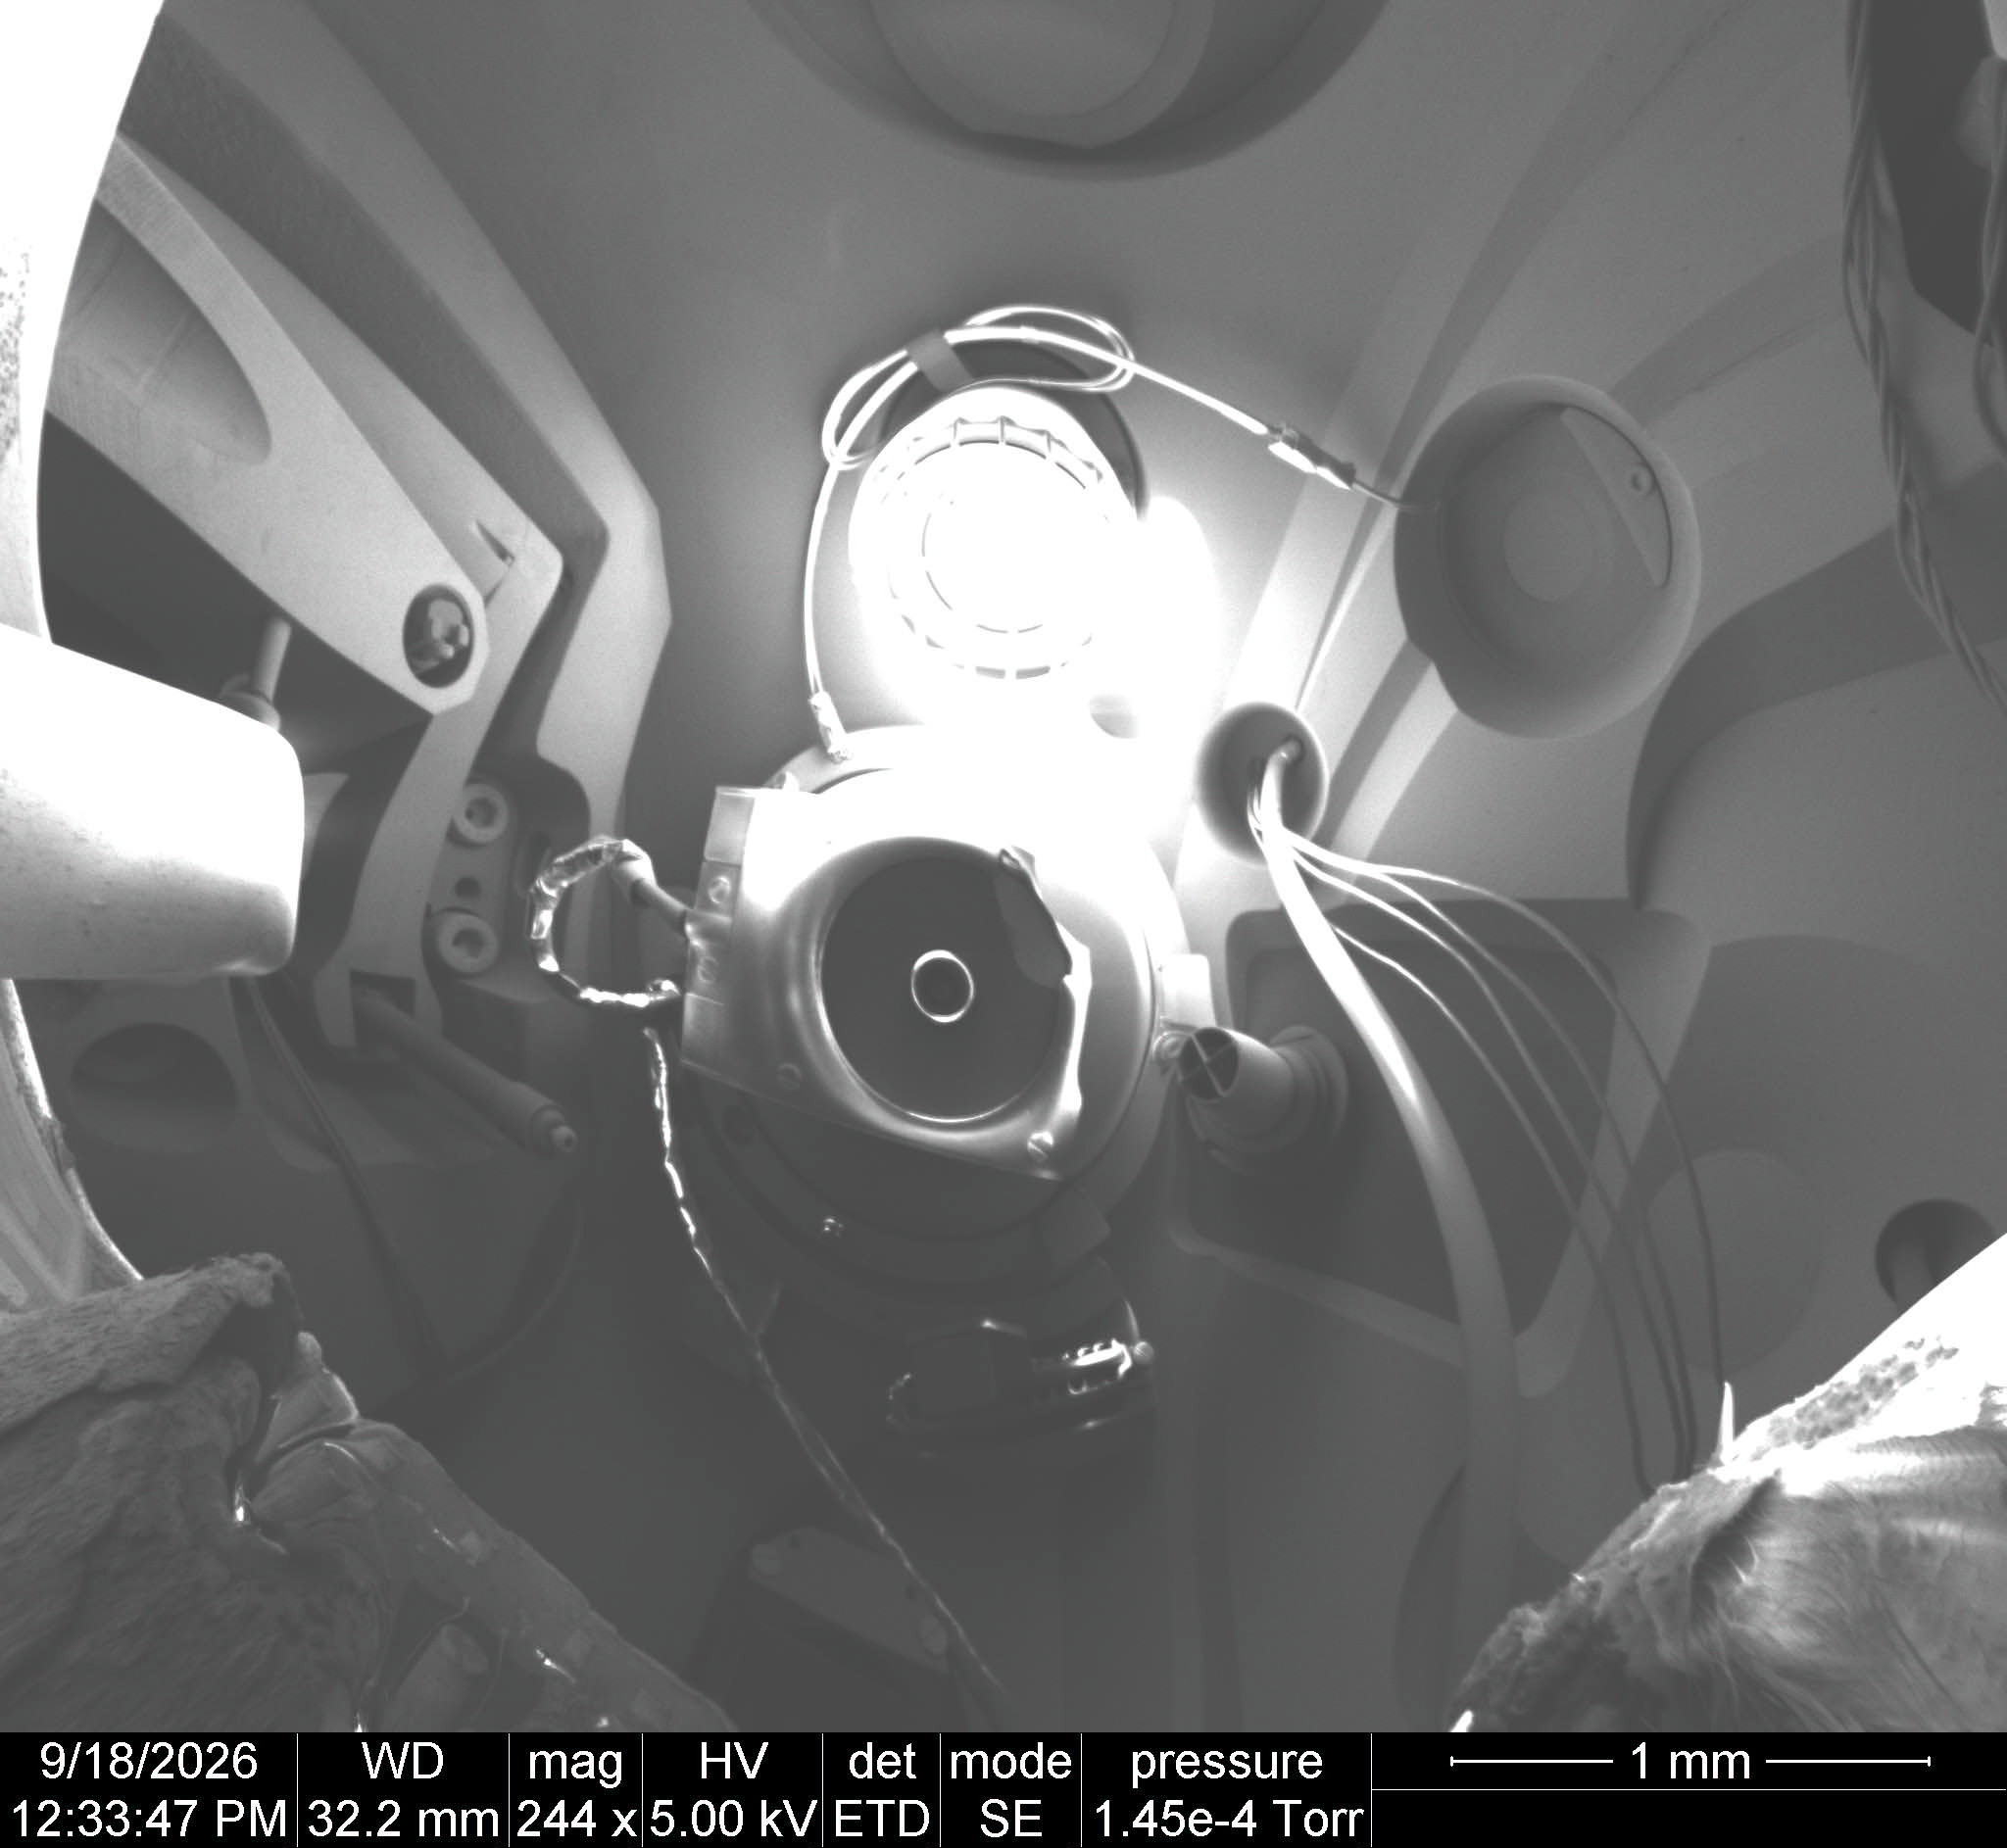
\includegraphics[width=0.5\textwidth]{000_004.jpg}
    \caption{Зеркальное изображение внутренней части колонны микроскопа.}
    \label{fig:mirror}
\end{figure}

% TODO: описать, какие элементы колонны микроскопа видны на зеркальном
% изображении (объективная линза, диафрагма и т.д.)



\subsection*{Зависимость коэффициента вторичной эмиссии от ускоряющего напряжения}

Целью данного этапа работы являлось экспериментальное определение коэффициента вторичной электронной эмиссии $\sigma$ и исследование его зависимости от ускоряющего напряжения $U$. 

Коэффициент вторичной эмиссии определялся по формуле:
\begin{equation}
    \sigma = \frac{I_{\text{отв}} - I_{\text{пов}}}{I_{\text{отв}}},
\end{equation}
где $I_{\text{отв}}$ --- ток, измеренный коллектором, расположенным под отверстием в цилиндре (аналог анализатора характеристического тока), а $I_{\text{пов}}$ --- ток, измеренный коллектором под поверхностью стенок цилиндра. Разность этих токов соответствует току вторичных электронов, выбитых с поверхности и не попавших в отверстие.

Измерения проводились в диапазоне ускоряющих напряжений от 0,5 до 30 кВ. Абсолютная инструментальная погрешность измерения токов составляла $\Delta I = 1$ пА ($0{,}001$ нА). Погрешность вычисляемого коэффициента $\Delta \sigma$ находилась по следующей формуле:
\begin{equation}
    \Delta \sigma = \sqrt{ \left( \frac{\partial \sigma}{\partial I_{\text{пов}}} \Delta I \right)^2 + \left( \frac{\partial \sigma}{\partial I_{\text{отв}}} \Delta I \right)^2 } = \frac{\Delta I}{I_{\text{отв}}} \sqrt{ 1 + \left( \frac{I_{\text{пов}}}{I_{\text{отв}}} \right)^2 }.
\end{equation}

Результаты измерений и расчётов представлены в таблице~\ref{tab:sigma_data}.

\begin{table}[h]
    \centering
    \caption{Зависимость коэффициента вторичной эмиссии $\sigma$ от ускоряющего напряжения}
    \label{tab:sigma_data}
    \begin{tabular}{|c|c|c|c|c|c|}
        \hline
        $U$, кВ & $I_{\text{пов}}$, нА & $I_{\text{отв}}$, нА & $\Delta I$, пА & $\sigma$ & $\Delta \sigma$ \\
        \hline
        30,0 & 0,444 & 0,570 & 1 & 0,2211 & 0,0022 \\
        25,0 & 0,357 & 0,469 & 1 & 0,2388 & 0,0027 \\
        20,0 & 0,307 & 0,395 & 1 & 0,2228 & 0,0032 \\
        17,0 & 0,267 & 0,345 & 1 & 0,2261 & 0,0037 \\
        15,0 & 0,286 & 0,370 & 1 & 0,2270 & 0,0034 \\
        12,0 & 0,285 & 0,367 & 1 & 0,2234 & 0,0034 \\
        10,0 & 0,243 & 0,310 & 1 & 0,2161 & 0,0041 \\
        5,0 & 0,239 & 0,300 & 1 & 0,2033 & 0,0043 \\
        2,0 & 0,296 & 0,349 & 1 & 0,1519 & 0,0038 \\
        1,5 & 0,283 & 0,326 & 1 & 0,1319 & 0,0041 \\
        1,0 & 0,298 & 0,332 & 1 & 0,1024 & 0,0040 \\
        0,5 & 0,095 & 0,100 & 1 & 0,0500 & 0,0049 \\
        \hline
    \end{tabular}
\end{table}

На рис.~\ref{fig:sigma_plot} представлена графическая зависимость коэффициента $\sigma$ от ускоряющего напряжения $U$.

\begin{figure}[h]
    \centering
    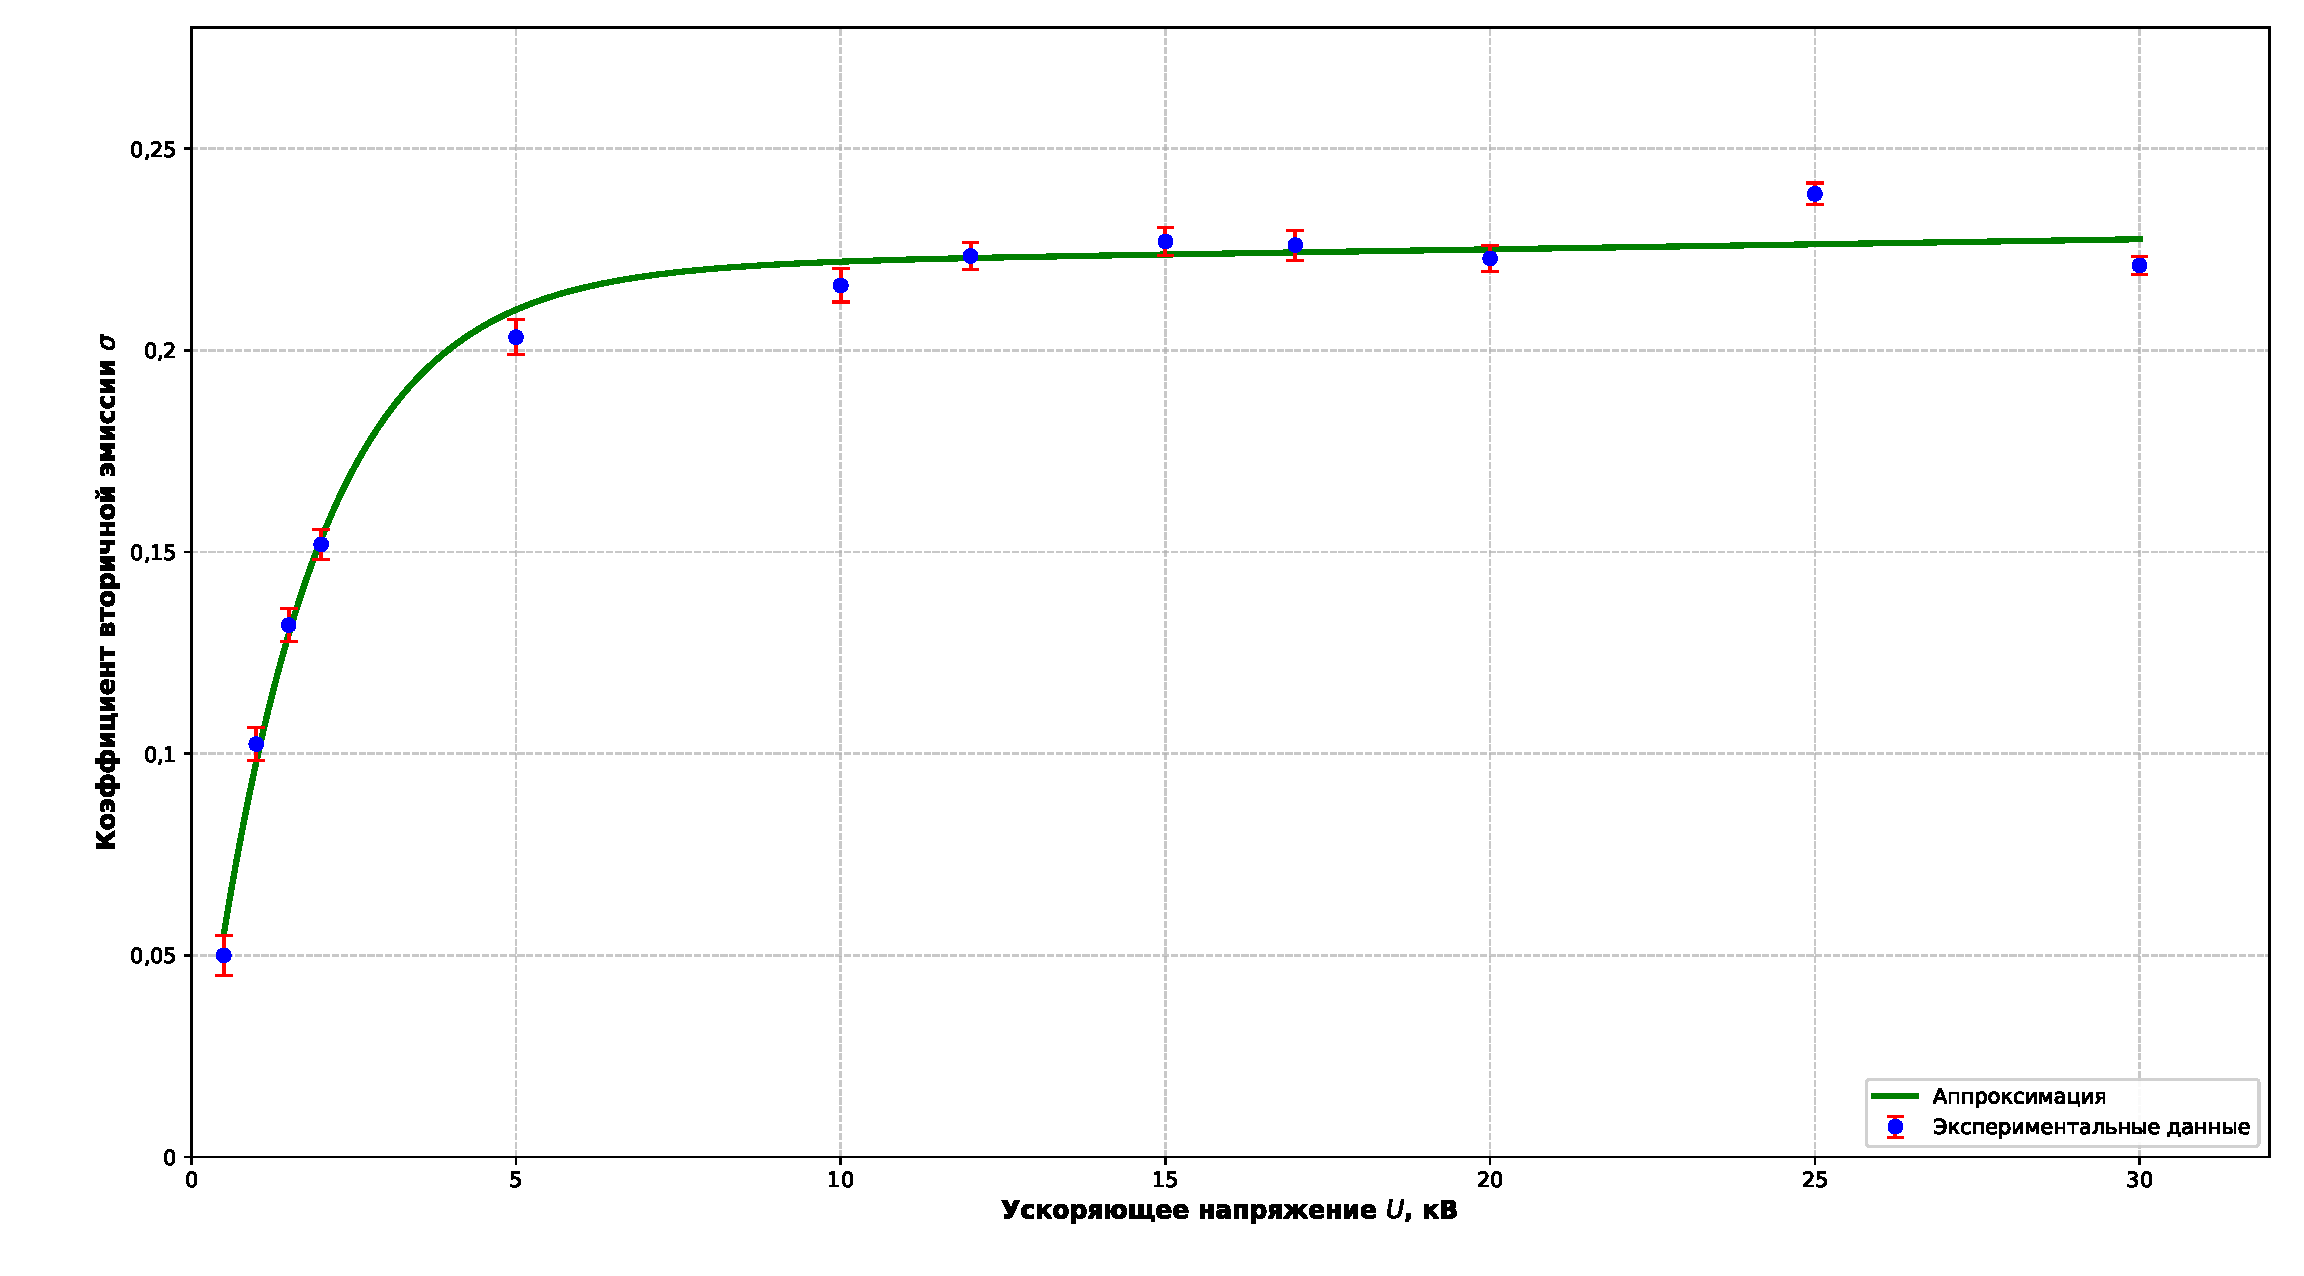
\includegraphics[width=0.7\textwidth]{График.pdf}
    \caption{Зависимость коэффициента вторичной эмиссии $\sigma$ от ускоряющего напряжения $U$.}
    \label{fig:sigma_plot}
\end{figure}

\newpage
\subsection*{Вывод}

В ходе выполнения лабораторной работы были изучены основные принципы работы растрового электронного микроскопа и методы формирования изображения. Экспериментально подтверждены различия между топографическим (SE, BSE A-B) и элементным (BSE A+B) контрастами. При исследовании диэлектрического образца (пенопластового шарика) было зафиксировано явление электростатической зарядки и эффект «электронного зеркала».

В заключительной части работы была исследована зависимость коэффициента вторичной электронной эмиссии $\sigma$ от ускоряющего напряжения в диапазоне от $0{,}5$ до $30$~кВ. Экспериментально подтверждено существование двух характерных участков на зависимости $\sigma(U)$:

\begin{itemize}
    \item области роста коэффициента при низких напряжениях ($0{,}5$--$5$~кВ), что объясняется увеличением глубины проникновения первичных электронов и ростом числа вторичных электронов, способных выйти на поверхность;
    
    \item области насыщения ($5$--$25$~кВ), где коэффициент достигает максимального значения $\sigma_{\text{max}} \approx 0{,}24$ и остаётся практически постоянным;
    
    % \item области возможного спада при высоких напряжениях ($> 25$~кВ), связанной с тем, что первичные электроны проникают слишком глубоко, и вторичные электроны не успевают достичь поверхности из-за неупругого рассеяния.
\end{itemize}

Полученная экспериментальная зависимость качественно согласуется с теоретическими представлениями о механизме вторичной электронной эмиссии. %Погрешность измерений $\Delta \sigma$ не превышала $0{,}004$ в основной части диапазона, что свидетельствует о хорошей воспроизводимости результатов.








\end{document}